%----------------------------------------------------------------------------------------
%	Metropolia Thesis LaTeX Template
%----------------------------------------------------------------------------------------
% License:
% This work is licensed under the Creative Commons Attribution 4.0 International License. 
% To view a copy of this license, visit http://creativecommons.org/licenses/by/4.0/.
%
% However, this license apply to this template. As a template, it is supposed to be 
% modified for your own needs (with your thesis content). For this reason, if you use 
% this project as a template and not specifically distribute it as part of a another 
% package/program, we grant the extra permission to freely copy and modify these files as 
% you see fit and even to delete this copyright notice. 
% In short, you are free to publish your thesis under whatever license you wish, even 
% keep the all rights reserved to you.
%
% Authors:
% Panu Leppäniemi, Patrik Luoto and Patrick Ausderau
%
% Credits:
% Panu Leppäniemi: abstract, def, cleaning,...
% Patrik Luoto: title page, abstract in Finnish, abbreviation, math,...
% Patrick Ausderau: initial version, style, table of content, bibliography, figure, 
%                   appendix, table, source code listing...
%
% Please:
% If you find mistakes, improve this template and alike, please contribute by sharing 
% your improvements and/or send us your feedback there: 
% https://github.com/panunu/metropolia-thesis-latex
% And of course, if you improve it, add yourself as an author.
%
% Compiler:
% Use XeLaTeX as a compiler.

%----------------------------------------------------------------------------------------
%	THESIS INFO
%----------------------------------------------------------------------------------------

% All general information (main language, title, author (you), degree programme, major 
% option, etc.)
% Edit the file chapters/0info.tex to change these information
% Global information (title of your thesis, your name, degree programme, major, etc.) 

\def\thesislang{english} %change this depending on the main language of the thesis. 
%\def\thesislang{english} % "english" is the only other supported language currently. If someone has the swedish, please contribute!

\def\secondlang{finnish} %if the main language is Finnish (or Swedish), you must have 2 abstracts (one in Finnish (or Swedish) and one in English)
%\def\secondlang{finnish} 
%If the main language is English and that you are native Finnish (or Swedish) speaker, you must have also abstract in your native language on top of the English one.

\author{Elisa Urjansson} %your first name and last name
\def\thesisfi{Insinöörityö}%was Opinnäytetyö
\def\thesisen{Thesis}

\def\alaotsikko{Alaotsikko/Subtitle} %DISABLED, seems not to be an option with the new template (2018). If you really need it, uncomment and modify style/title.tex accordingly %if you don't have subtitle, empty {} it (but don't delete that line)

%Finnish section, for title/abstract
\def\otsikko{LoRa laitteiden autentikaation automatisointi langattomasti Robot Frameworkilla}
\def\tutkinto{Insinööri (AMK)} % change to your needs, e.g. "YAMK", etc.
\def\kohjelma{Tieto\textendash ja viestintätekniikka}
\def\suuntautumis{Älykkäät järjestelmät}
\def\ohjaajat{
Projekti-insinööri Joseph Hotchkiss\newline
}
\def\avainsanat{LoRa, IoT, Robot Framework, ohjelmistorobotiikka, ChirpStack}
\def\pvm{\specialdate\today}

%English section, for title/abstract
\title{Robot Framework automation for OTAA of LoRa devices}
\def\metropoliadegree {Bachelor of Engineering} % change to your needs, e.g. "master", etc.
\def\metropoliadegreeprogramme {Information and Communication Technology}
\def\metropoliaspecialisation {Smart Systems}
\def\metropoliainstructors {
Joseph Hotchkiss, Project Engineer\newline
}
\def\metropoliakeywords {LoRa, Internet of Things, Robot Framework, Robotic Process Automation, ChirpStack}
\date{\longmonth\today}




%----------------------------------------------------------------------------------------
%	GLOBAL STYLES
%----------------------------------------------------------------------------------------

% If you need extra package, etc. modify the style/style.tex file.
% If you are using Windows OS, you will need to change default font to Arial in that 
% style/style.tex file (or install Liberation Sans font to your system).
% If you are using MacOS or linux, make sure you have Liberation Sans font installed.
% Global style. Normally should not be edited. 
% If you use windows OS, eventually change \setmainfont to Arial
% Check around commit https://github.com/panunu/metropolia-thesis-latex/commit/a0c15ac77bab1a52c59c517a18080938e57bf5ef
% to see how the font files were manually added (after downloading them: https://pagure.io/liberation-fonts/ )

\documentclass[11pt,a4paper,oneside,article]{memoir}
\usepackage{xcolor}
\newcommand\todo[1]{\textcolor{red}{TODO: #1}}
\usepackage[\secondlang,\thesislang]{babel}% finnish english swedish
\usepackage{iflang}
\usepackage{amsmath}
\usepackage{amsfonts}
\usepackage{amssymb}
\usepackage{fontspec}
\usepackage{tocloft}
\usepackage{titlesec}
\usepackage[hyphens]{url}
\usepackage{mathtools}
\usepackage{wallpaper}
\usepackage{datetime}
\usepackage[bookmarksdepth=subsection]{hyperref} % for automagic pdf links for toc, refs, etc.
\usepackage[amssymb]{SIunits}
\usepackage[version=3]{mhchem}
\usepackage{pgfplots} %simple plots etc
\usepackage{pgfplotstable}
\usepackage{tikz} % mindmaps, flowcharts, piecharts, examples at http://www.texample.net/tikz/examples/
\usetikzlibrary{shapes.geometric, arrows}


\renewcommand{\dateseparator}{.}
%condition for adding or not space in TOC
\usepackage{etoolbox}
%for compact list
\usepackage{enumitem}
%for block comment
\usepackage{verbatim}
%for "easier" references
\usepackage{varioref}
%forcing single line spacing in bibliography
\DisemulatePackage{setspace}
\usepackage{setspace}
%including figure (image)
\usepackage{graphicx}
%change the numbering for figure
\usepackage{chngcntr}
%strike trough
\usepackage{ulem}
%euro symbol
\usepackage{eurosym}
%try to count
\usepackage{totcount}
%insert source code
%\usepackage{listings}
%require -8bit -shell-escape in the xelatex compile command
%if compiling locally, consider options cachedir=minted,outputdir=~/.tex
\usepackage[newfloat]{minted}
\setminted{tabsize=2,linenos,breaklines,breaksymbolleft={\quad},baselinestretch=1}
\setmintedinline{breaklines}
\usepackage[justification=justified,singlelinecheck=false,font=small]{caption}
\usepackage{color}
%force the width of a table instead of column
\usepackage{tabularx}
\usepackage{booktabs} %why not booktabs? :3
% Abbreviations, acronym and glossary
\usepackage[acronym,toc,nonumberlist,section=chapter]{glossaries}%xindy,%toc, ,nomain
\renewcommand*{\glsclearpage}{}

\usepackage{float} % For forced figure location with modifier H (\begin{figure}[H])
\usepackage{cite} % Make citations to match Metropolia thesis guide

% change font of links in bibliography to same as other text
\usepackage{url}
\urlstyle{same}

% change punctuation of multiple cites to semicolon instead of comma: [1; 2; 3]
\renewcommand\citepunct{; }

% citep-macro for reference with period inside square brackets [1.]
\newcommand{\citep}[1]{
 \renewcommand\citeright{.]}
 \cite{#1}
 \renewcommand\citeright{]}
}

%set date format to D.M.YYYY
\newdateformat{specialdate}{\THEDAY.\THEMONTH.\THEYEAR}
%set date format to D Month YYYY
\newdateformat{longmonth}{\THEDAY~\monthname[\THEMONTH] \THEYEAR}

\newcommand\tn[1]{\textnormal{#1}} %use \tn instead of \textnormal
\newcommand\reaction[1]{\begin{equation}\ce{#1}\end{equation}} %\reaction{} for chemical reactions

%NORMAL TEXT
%all text, title, etc. in the same font: Arial
%NOTE: fontname is case-sensitive
\setmainfont{Liberation Sans}
%line space
\linespread{1.5}
\AtBeginEnvironment{tabular}{\singlespacing}
%\doublespacing
%margin
\usepackage[top=2.5cm, bottom=3cm, left=4cm, right=2cm, nofoot]{geometry}
\setlength{\parindent}{0pt} %first line of paragraph not indented
\setlength{\parskip}{16.5pt} %one empty line to separate paragraph
%list with small line space separation
\tightlists

%IMAGE - FIGURE
%the figures should be placed in the "illustration" folder
\graphicspath{{illustration/}}
%figure number without chapter (1.1, 1.2, 2.1) to (1, 2, 3)
\counterwithout{figure}{chapter}
%border around images
\setlength\fboxsep{0pt}
\setlength\fboxrule{0.5pt}
%space after figure caption (and other float elements)
\setlength{\belowcaptionskip}{-7pt}

%TABLE
\counterwithout{table}{chapter}

%SOURCE CODE
\newenvironment{code}{\captionsetup{type=listing}}{}
\IfLanguageName {finnish} {\SetupFloatingEnvironment{listing}{name=Koodiesimerkki}} {}%was Listaus
%\counterwithout{lstlisting}{chapter}
%moved after begin document, otherwise does not compile

%% set this format as the default for lstlisting
%\DeclareCaptionFormat{empty}{}
%\captionsetup[lstlisting]{format=empty}

%TOC
%change toc title
\IfLanguageName {finnish} {\addto{\captionsfinnish}{\renewcommand*{\contentsname}{Sisällys}}} {}
%remove dots
\renewcommand*{\cftdotsep}{\cftnodots}
%chapter title and page number not in bold
\renewcommand{\cftchapterfont}{}
\renewcommand{\cftchapterpagefont}{}
%sub section in toc
\setcounter{tocdepth}{2}
%subsection numbered
\setcounter{secnumdepth}{2}
\renewcommand{\tocheadstart}{\vspace*{-15pt}}
\renewcommand{\printtoctitle}[1]{\fontsize{13pt}{13pt}\bfseries #1}
%\renewcommand{\aftertoctitle}{\vspace*{-22pt}\afterchaptertitle}
%spacing afer a chapter in toc
\preto\section{%
  \ifnum\value{section}=0\addtocontents{toc}{\vskip11pt}\fi
}
%spacing afer a section in toc
\renewcommand{\cftsectionaftersnumb}{\vspace*{-3pt}}
%spacing afer a subsection in toc
\renewcommand{\cftsubsectionaftersnumb}{\vspace*{-1pt}}
%appendix in toc with "Appendix " + num
\IfLanguageName {finnish} {
  \renewcommand*{\cftappendixname}{Liite\space}
  \renewcommand{\appendixtocname}{Liitteet}
}{\renewcommand*{\cftappendixname}{Appendix\space}}
%appendix header
\IfLanguageName {finnish} {\def\appname{Liite\space}}{\def\appname{Appendix\space}}

%TITLES
%chapter title
%\clearforchapter{\clearpage}
\titleformat{\chapter}
{\fontsize{13pt}{13pt}\bfseries\linespread{1}}%\clearpage
{\thechapter}{.5cm}{}
\titlespacing*{\chapter}{0pt}{.32cm}{9pt}
\titleformat{\section}
{\fontsize{12pt}{12pt}\linespread{1}}
{\thesection}{.5cm}{}
\titlespacing*{\section}{0pt}{14pt}{6pt}
\titleformat{\subsection}
{\fontsize{12pt}{12pt}\linespread{1}}
{\thesubsection}{.5cm}{}
\titlespacing*{\subsection}{0pt}{14pt}{6pt}


%QUOTE
\renewenvironment{quote}
  {\list{}{\rightmargin=0pt\leftmargin=1cm\topsep=-10pt}%
  \item\relax\fontsize{10pt}{10pt}\singlespacing}
  {\endlist}

%BIBLIOGRAPHY
%bibliography title to be "references"
%IF THE TITLE DON'T GET RENAMED PROPERLY, move that line after the \begin{document}
\IfLanguageName {finnish} {\addto{\captionsfinnish}{\renewcommand*{\bibname}{Lähteet}}} {\renewcommand\bibname{References}}
\makeatletter %reference list option change
\renewcommand\@biblabel[1]{#1\hspace{1cm}} %from [1] to 1 with 1cm gap
\makeatother %
\setlength{\bibitemsep}{11pt}

%count the appendices (since the chapter counter is reset after \appendix).
%! require to complie 2 times
\regtotcounter{chapter}


\makepagestyle{tiivis}
\makeevenhead{tiivis}{}{}{Tiivistelmä}
\makeoddhead{tiivis}{}{}{Tiivistelmä}

\makepagestyle{abstract}
\makeevenhead{abstract}{}{}{Abstract}
\makeoddhead{abstract}{}{}{Abstract}

%footer on every pages
\LLCornerWallPaper{1}{\IfLanguageName{finnish}{footer_fi}{footer_en}}

% Normally, you do not need to modify the title style. It's content comes from the 
% chapters/0info.tex file.
% TITLE PAGE
% Normally, you should not edit this file.

\makeatletter
\renewcommand{\maketitle}{
\newgeometry{left=4.5cm}
\thispagestyle{empty}
\ThisULCornerWallPaper{1}{\IfLanguageName{finnish}{metropolia_fi}{metropolia_en}}
%
\vspace*{12.8cm}
\tn{\Large\@author\\[1cm]\Huge\IfLanguageName {finnish}{\color[RGB]{155,50,35}\otsikko}{\color[RGB]{31,73,125}\@title}}%\\[22pt]\LARGE\alaotsikko\\[1.75cm]}

\null\vfill
\parbox{.7\linewidth}{
\IfLanguageName {finnish}{
  Metropolia Ammattikorkeakoulu\\
  \tutkinto \\
  \kohjelma \\
  \thesisfi\\
  \pvm
} {
  Helsinki Metropolia University of Applied Sciences\\
  \metropoliadegree \\
  \metropoliadegreeprogramme \\
  \thesisen\\
  \IfLanguageName {finnish}{\pvm}{\@date} % D.M.YYYY date format for Finnish. D Month YYYY for English
}
}
\vspace*{-1.5cm}
\clearpage
\restoregeometry
}
\makeatother



%----------------------------------------------------------------------------------------
%	ABBREVIATION AND GLOSSARY
%----------------------------------------------------------------------------------------

% Add/edit all your acronyms, abbreviations, glossary entries, etc. definitions in 
% chapters/0abbr.tex file.
% You can have as many as you wish. Only the ones you use in your text (inserted with 
% \gls{} command) will print in the Glossary/Lyhenteet.
% Generate the glossary
\makeglossaries

% Acronyms, abbreviations, etc. 


\newacronym{rpa}{RPA}{Robotic Process Automation}
\newacronym{iot}{IoT}{Internet of Things}
\newacronym{otaa}{OTAA}{Over The Air Activation}
\newacronym{lora}{LoRa}{Low Range}
\newacronym{lorawan}{LoRaWAN}{Low Range Wide Area Network}
\newacronym{ui}{UI}{User Interface}
\newacronym{fuota}{FUOTA}{Firmware Update Over the Air}
\newacronym{url}{URL}{Uniform Resource Locator}
\newacronym{sd}{SD}{Secure Digital}
\newacronym{os}{OS}{Operating System}
\newacronym{ssh}{SSH}{Secure Shell}
\newacronym{abp}{ABP}{Activation by Personalization}
\newacronym{eirp}{EIRP}{Equivalent Isotopically Radiated Power}
\newacronym{mac}{MAC}{Media Access Control}
\newacronym{ttl}{TTL}{time-to-live}
\newacronym{mqtt}{MQTT}{Message Queuing Telemetry Transport}
\newacronym{http}{HTTP}{HyperText Transfer Protocol}
\newacronym{rest}{REST}{REpresentational State Transfer}
\newacronym{api}{API}{Application Programming Interface}
\newacronym{grpc}{gRPC}{Remote Procedure Call}
\newacronym{db}{DB}{Database}
\newacronym{ip}{IP}{Internet Protocol}
\newacronym{ca}{CA}{Certificate Authority}
\newacronym{tls}{TLS}{Transport Layer Security}
\newacronym{eui}{EUI}{Extended Unique Identifier}
\newacronym{cli}{CLI}{Command Line Interface}
\newacronym{sdk}{SDK}{Software development kit}
\newacronym{pdf}{PDF}{Portable Document Format}

% Glossary entries

\newglossaryentry{part_key}{
	name={partition key}, 
	description={a column or set of columns from the same table whose consolidated value decide the partition for a given data}
}
\newglossaryentry{thesis}{
	name=thesis, 
	description={a written essay one submitted for a university degree},
	plural=theses
}
\newglossaryentry{latex}
{
    name=\LaTeX{},
    description={Is a mark up language specially suited for scientific documents}
}
 
\newglossaryentry{maths}
{
    name=mathematics,
    description={Mathematics is what mathematicians do}
}




%----------------------------------------------------------------------------------------
%	DOCUMENT STARTS HERE...
%----------------------------------------------------------------------------------------

\begin{document}
\counterwithout{listing}{chapter}

%----------------------------------------------------------------------------------------
%	TITLE PAGE
%----------------------------------------------------------------------------------------

% Title header. You should not edit that file.

%page number always on the top right, clear the "chapter/section" head
\pagestyle{myheadings}
\markright{}
%clear chapter "title" foot page
\makeevenfoot{plain}{}{}{}
\makeoddfoot{plain}{}{}{}



\maketitle
\newpage

%----------------------------------------------------------------------------------------
%	ABSTRACT / Tiivistelmä
%----------------------------------------------------------------------------------------

% If you are international student writing in English, remove the Finnish abstract.
% If you are Finnish citizen, you must have 2 abstracts, one in Finnish (or Swedish 
% depending on your mother tongue) and one in English regardless of the main language of 
% your thesis.
% Abstract in Finnish
%Most probably, you only need to change the text of the abstract. Everything else comes from chapter/0info.tex
%If you do not have any appendix, you may delete \total{chapter} and replace with 0

\thispagestyle{tiivis}
\begin{otherlanguage}{finnish}
{\renewcommand{\arraystretch}{2}%
\begin{tabular}{ | p{4,7cm} | p{10,3cm} |}
  \hline
  Tekijä(t) \newline
  Otsikko \newline\newline 
  Sivumäärä \newline
  Aika
  & 
  \makeatletter
  \@author \newline 
  \otsikko \newline\newline %! if very long title over 2 lines, remove one \newline
  \makeatother
  \pageref*{LastPage} sivua + \total{chapter} liitettä \newline %! if no appendices, risk to count total of chapter :D
  \pvm		
  \\ \hline
  Tutkinto & \tutkinto
  \\ \hline
  Tutkinto-ohjelma & \kohjelma
  \\ \hline
  Ammatillinen pääaine & \suuntautumis
  \\ \hline
  Ohjaaja(t) & \ohjaajat
  \\ \hline
  \multicolumn{2}{|p{15cm}|}{\vspace{-22pt}
  Robot Framework on avainsanaohjattu avoimen lähdekoodin automaatiokehys, jota voidaan käyttää testiautomaatioon ja  ohjelmistorobotiikkaan. Se on laajennettavissa useilla kirjastoilla, jotka voidaan totetuttaa eri ohjelmointikielillä ja sen syntaksi käyttää luettavia avainsanoja. \newline

  Tämä opinnäytetyö perustuu Robot Framework automaatio- toteutukseen \gls{lora} laitteille, jotka käyttävät \gls{otaa} metodia palvelimen kanssa kommunikointiin ja opinnäytetyö suoritettiin Metropolia Ammattikorkeakoululle. Materiaali työhön kerättiin tutkimalla verkkomateriaalia Robot Frameworkille tarjolla olevista kirjastoista, perehtymällä yksityiskohtaisempaan materiaaliin liittyen ChirpStack verkkopalvelimeen ja LORIX One reitittimeen, sekä tutkimalla Metropoliassa aiemmin opiskelleen henkilön opinnäytetyöhön, jossa \gls{lora} päätelaite oli kehitetty. Opinnäytetyön toteutusta testattiin kehityksen ohessa ajamalla ohjelmakoodia ja varmistamalla että yhteydet laitteen, palvelimen ja reitittimen välillä toimivat asianmukaisesti. \newline

  Toteutus tarjoaa ohjelmakoodin, joka lisää \gls{lora} päätelaitteen äskettäin luotuun sovellukseen ChirpStack verkkopalvelimeen, mihin laitteilla on yhteys   \gls{otaa} metodin avulla käyttämällä LORIX One reititintä \gls{lorawan} protokollalla. \newline

  Tämän opinnäytetyön lopputulos auttaa Metropolia Ammattikorkeakoulua poistamalla toistuvia tehtäviä, joita opettajien on tarvinnut tehdä langattomien teknologioiden kurssien alussa ja siten tarjoamalla enemmän aikaa kohdennettavaksi opetustoimintaan. \newline
  } \\[14cm] \hline
  Avainsanat & \avainsanat
  \\ \hline
\end{tabular}
}
\end{otherlanguage}
\clearpage


\glsresetall
% Abstract in English
%Most probably, you only need to change the text of the abstract. Everything else comes from chapter/0info.tex
%If you do not have any appendix, you may delete \total{chapter} and replace with 0

\pagestyle{abstract}
\begin{otherlanguage}{english}
{\renewcommand{\arraystretch}{2}%
\begin{tabular}{ | p{4,7cm} | p{10,3cm} |}
  \hline
  Author(s) \newline
  Title \newline\newline 
  Number of Pages \newline
  Date
  & 
  \makeatletter
  \@author \newline
  \@title \newline\newline %! if very long title over 2 lines, remove one \newline
  \pageref*{LastPage} pages + \total{chapter} appendices \newline %! if no appendices, risk to count total of chapter :D
  \IfLanguageName {finnish} {\foreignlanguage{english}{\longdate\@date}} {\@date}
  \makeatother
  \\ \hline
  Degree & \metropoliadegree
  \\ \hline
  Degree Programme & \metropoliadegreeprogramme
  \\ \hline
  Professional Major & \metropoliaspecialisation
  \\ \hline
  Instructor(s) & \metropoliainstructors
  \\ \hline
  \multicolumn{2}{|p{15cm}|}{\vspace{-22pt}
  Abstract content. To force newline between paragraph in the abstract, you must have both a empty line and the newline command. \newline

  beginning of second paragraph\ldots
  } \\[14cm] \hline
  Keywords & \metropoliakeywords
  \\ \hline
\end{tabular}
}
\end{otherlanguage}
\clearpage



%----------------------------------------------------------------------------------------
%	License? Acknowledgement?
%----------------------------------------------------------------------------------------

% Uncomment next line and edit chapters/0license.tex if you want license in your thesis.
%% License of your thesis
% If you wish to explain what it means. When you publish your thesis in https://theseus.fi
% you will be able to choose between some Creative Commons licenses 
% https://creativecommons.org
% Adapt this example text to your taste.
% This would also be the right place to explain the license you choose for the code you 
% produced for your thesis.

\pagestyle{empty}
\chapter*{Licenses}
\vspace{-20pt}
\begin{center}
 
\includegraphics[width=80pt]{cc_by_sa}
\end{center}\vspace{-32pt}
This work is licensed under the Creative Commons Attribution-ShareAlike 4.0 International License. That means:\\
\textbf{You are free to:}
\vspace{-17pt} \begin{itemize}
\item Share \textemdash copy and redistribute the material in any medium or format
\item Adapt \textemdash remix, transform, and build upon the material
\end{itemize}\vspace{-17pt}

\textbf{Under the following terms:}
\vspace{-17pt} \begin{itemize}
\item Attribution \textemdash You must give appropriate credit, provide a link to the license, and indicate if changes were made. You may do so in any reasonable manner, but not in any way that suggests the licensor endorses you or your use.
\item ShareAlike \textemdash If you remix, transform, or build upon the material, you must distribute your contributions under the same license as the original.
\item No additional restrictions \textemdash You may not apply legal terms or technological measures that legally restrict others from doing anything the license permits.
\item Any of the above conditions can be waived if you get my permission
\end{itemize}%\vspace{-17pt}


To view a copy of this license, visit \url{http://creativecommons.org/licenses/by-sa/4.0/}.

I decided to publish my thesis work under the Creative Commons Attribution-ShareAlike 4.0 International License because I strongly believe that you as reader deserve the freedom to copy, share and modify this work and if you do modify it, it is fair to give these same permissions to the others. A copy in electronic form of this work can be found in \url{https://some.place} with the \LaTeX{} source.

\clearpage


% Uncomment next line and edit chapters/0acknowledgement.tex if you want acknowledgements.
%% Acknowledgement
% If relevant give a special thanks to the people who supported you during your thesis 
% writing. 

\pagestyle{empty}
\chapter*{Acknowledgement}

Thanks to Panu Leppäniemi, Patrik Luoto and Patrick Ausderau for the \LaTeX{} ~thesis template.

Thanks to my cat who jump on my keyboard while the text was not saved :D

\clearpage



%----------------------------------------------------------------------------------------
%	TABLE OF CONTENTS
%----------------------------------------------------------------------------------------

% Table of Content
% Normally, you don't have to modify this file.
% In case spacing of appendix/liite goes crazy, look in ../thesis.tex and look
% for the hack described in APPENDICES.

\makeevenhead{plain}{}{}{}
\makeoddhead{plain}{}{}{}
\pagestyle{empty} %remove page number in toc (if longer than 2 pages)
\tableofcontents*
\pagestyle{empty} %remove page number in toc (if longer than 1 pages)

\clearpage



%list of figure, tables would come here if relevant?

%----------------------------------------------------------------------------------------
%	Lyhenteet / Abbreviation
%----------------------------------------------------------------------------------------

% If you don't use abbreviations/glossary, remove the following line.
% Abbreviation and Glossary
% Normally, you don't have to modify this file. Your abbreviations, etc. goes in 
% ../chapters/0abbr.tex file.

\begin{singlespacing}

% \gsladdall would add all terms even if not used in your text.
%\glsaddall
  \addtocontents{toc}{\cftpagenumbersoff{chapter}}
{
	\titleformat{\section}
	{\fontsize{13pt}{13pt}\bfseries\linespread{1}}
	{\thesection}{.5cm}{}
	%Adapt labelwidth (sorry for the ugly hack)
	\setlist[description]{leftmargin=!, labelwidth=4em}
	\IfLanguageName {finnish} {
		\printacronyms[title=Lyhenteet]
	}{
		\printacronyms[title=List of Abbreviations]
	}
	\setlist[description]{leftmargin=!, labelwidth=7em}
	\printglossary 
	\setlist[description]{style=standard} % reset settings back to default
}
\addtocontents{toc}{\cftpagenumberson{chapter}} 
\end{singlespacing}

\clearpage


%----------------------------------------------------------------------------------------
%	CONTENT
%----------------------------------------------------------------------------------------

% Style for the main thesis content.
% Normally, you should not edit this file.

%page number always on top right; also for chapter "title" page
\pagestyle{plain}
\makeevenhead{plain}{}{}{\thepage}
\makeoddhead{plain}{}{}{\thepage}

\setcounter{page}{1} %page 1 should be Introduction

\sloppy % enforce alignment to fully justified


%reset page number to 1, etc.

% Thesis content if you strictly follow the "Final Year Project guide". Of course, you 
% can adapt to your specific needs (add more chapter, rename them, etc.).
\glsresetall
% Introduction

\chapter{Introduction}

In the swiftly moving field of technology, automation is increasing widely, offering advantages such as enhanced reliability, efficiency, and availability.
Two important thing in this field are  \gls{iot} and \gls{rpa}. Specifically, \gls{rpa} is a significant tool for making complicated tasks easier by efficiently handling repetitive tasks, while \gls{iot} enhances the overall environment by connecting devices and enabling smart functionalities. 

This thesis is presented to Metropolia University of Applied Sciences to benefit their courses that are related with the wireless technologies. In these courses the students utilize \gls{lora} end devices that have \gls{otaa} to establish connection to the LORIX One gateway. The gateway acts as the bridge, connecting the devices to the Chirpstack \gls{lorawan} network server. In the beginning of a course the teacher needs to create a new application to the server and add all the devices to that application. This includes a lot of repeating work that can be automated. The implementation seeks to minimize the time commitment from the teachers at the onset of each course by providing automation for data transcription. The objective is to enhance overall efficiency, enabling lecturers to allocate more attention to instructional activities.

This thesis contains 6 chapters.
Chapter~\ref{ch:theor_backgr} describes the theoretical foundation of the project, exploring potential alternatives to the chosen implementation method.
Chapter~\ref{ch:mat_met} presents detailed information on \gls{lorawan}, LORIX One, ChirpStack, and the Robot Framework and provides a comprehensive understanding of these key components.
Chapter~\ref{ch:project_spec} offers a detailed description of the project's specifications, offering a broad overview of the scope and requirements. 
Chapter~\ref{ch:impl} focuses on the practical aspects of the implementation process, offering a step-by-step breakdown.
Chapter~\ref{ch:conc} summarizes the findings and insights obtained throughout the entire thesis.


\clearpage %force the next chapter to start on a new page. Keep that as the last line of your chapter!

% uncomment what you need.
% Theoretical background

\chapter{Theoretical Background} \label{ch:theor_backgr}

This project was developed on top of another student's final year project \cite{theseus:gere-zoltan} to automate the tasks that are required in the beginning of each course that uses their implementation.
Their solution provided the \gls{lora} end device, ChirpStack network server and LORIX One Gateway as starting tools.
The following section is a walk-through of the features ChirpStack server's web-interface provides and how it is used without the implementation of automation this project provides.
The starting point of this walk-through occurs after the server has been set up and configured.

The end devices that the students use are added to an application in the ChirpStack server.
The server has a clear \gls{ui} which is opened to the Applications page when the user logs in as seen in Figure~\ref{fig:ChirpStack_application_list}.

\begin{figure}[ht]
  \centering
  {\includegraphics[width=\textwidth]{illustration/ChirpStack_application_list.png}}
  \caption{List of applications on a ChirpStack network server.}
  \label{fig:ChirpStack_application_list}
\end{figure}

The page layout provides a sidebar that can be hidden from view with an arrow button next to the ChirpStack logo.
The sidebar consists of two sections.
The first section contains four buttons: Network-servers, Gateway-profiles, Organizations, and All users
The second section includes a drop-down list to select an organization and seven additional buttons: Org. settings, Org. users, Service-profiles, Device-profiles, Gateways, Applications, and Multicast-groups.
Each button corresponds to a specific category or feature.
Clicking on any of these buttons navigates the user to a dedicated page or section displaying a list of elements associated with that category.
Each element in the list is hyperlinked to provide easy access to its details, allowing users to view and modify the information they have previously provided during creation or addition to the list.
Next, moving the layout and features of each button are discussed individually.

\section{Network-servers}
Network-servers display the added network servers, providing their names and server details in the hostname:port format.
Users can click the Add button to create a new network server to the list.
When creating a new server, users must provide a server name and specify the server details, including the hostname and port in a single field, as mandatory fields.
Additionally, users have the option to include additional features, such as enabling gateway discovery and providing \gls{ca} and \gls{tls} certificates, along with \gls{tls} keys for both ChirpStack Application Server to ChirpStack Network Server connection and vice versa, in the network server details.

\section{Gateway-profiles}
Gateway-profiles contain the added gateway-profiles.
To create a new one, a user presses the Add button and fills in the mandatory fields of the enabled channels, which can be separated with commas, and by choosing a network-server from a drop-down list.
The gateway-profiles are not used in the courses the school use the ChirpStack with, and the feature is also to be removed in ChirpStack's next major release, which is yet to have a release date.

\section{Organizations}
The Organizations layout consists of the inserted organizations to the ChirpStack.
The list view provides information of the organizations' name, display name and its possibility of having gateways.
Those details are also to be filled in if the user adds a new organization by clicking the Create button.

\section{All users}
All users consists of the users added to ChirpStack.
The list view shows the username, active status and admin privileges of the users.
A new user can be added by clicking the Create button and providing the mandatory fields of username, e-mail address and password.
Additional details are the optional note field and permission tick boxes which allow selecting if the user is active and giving global admin privileges.

When the user selects an organization from the second section's drop-down list, that organization's details are used with all the buttons below to check and modify the information on the layouts the buttons navigate to.

\section{Org. settings}
Org. settings is for updating the settings of the selected organization of the drop-down list.
Adjustable information is the same ones are used, when a new organization is created on the previously mentioned Organizations layout.

\section{Org. users}
Org. users is a layout where the users assigned to the selected organizations can be seen and new ones can be added.
The list view shows the ID of the user, their username and if the user has admin privilege on that organization.
The username is a hyperlink that directs to a layout where the username is seen and where the organization's admin privilege can be granted or removed.
The layout provides three buttons called Delete, Update user, and Goto user.
The Delete button removes a user from the organization.
The Update user button is used if changes to privilege has been made.
The Goto user button directs to a similar layout to what the All Users layout had for creating a new user with fields populated with the details given upon user creation.
\clearpage

\section{Service-profiles}
The Service-profiles layout provides a list of service profile names that are appended to the organization.
The name is a hyperlink that leads to a page where details can be updated.
When a new service-profile is added from the Create button a new layout opens.
Service profile creation requires a service-profile name and a network server from a drop-down list of servers that are part of the organization.
Additional details contain tickboxes to allowing to add gateway meta-data and to enable network geolocation.
In addition 3 fields can be ticked to give the device-status request frequency, minimum allowed data-rate and maximum allowed data-rate.

\section{Device-profiles}
Device-profiles is otherwise similar to the Service-profiles layout with the difference of the form of adding or modifying a device profile.
That form includes five tabs: general, join (\gls{otaa} / \gls{abp}), class-B, class-C and codec.
The general tab includes two mandatory text fields called Device-profile name and Max \gls{eirp} and an optional text field called Geolocation buffer \gls{ttl} (seconds). The view also has three mandatory drop-down list fields where the network-server, \gls{lorawan} \gls{mac} version and \gls{lorawan} Regional Parameters revision needs to be selected.
The form also contains a field where the Geolocation buffer \gls{ttl} can be selected.
A device profile can already be created after filling the general information, but if other features are to be added, all mandatory fields from that tab's layout needs to be filled.
The join (\gls{otaa} / \gls{abp}) tab has a tick box from where the user can select if the device supports \gls{otaa}.
The rest of the fields are mandatory and consist of four incremental input fields called RX1 delay, RX1 data-rate offset, RX2 data-rate, RX2 channel frequency (Hz), and a regular text field called Factory-preset frequencies (Hz).
The Class-B tab has one tick box which determines if the device supports Class-B.
The Class-C tab  has the same tick box, but for Class-C device support and also a mandatory incremental input field for Class-C confirmed downlink timeout.
The Codec tab provides an optional drop-down list for selecting the Payload codec.

\section{Gateways}
The Gateways layout provides a list view of the gateways that are added to the selected organization. 
It also delivers a Create button to add new gateways.
The list view has three items it shows of each gateway, the Name, Gateway ID, and Gateway activity (30d).
The name is a hyperlink from where the gateway details can be accessed and modified.
The Gateway ID gives the user a fast way to check the ID of the gateway. 
Gate activity (30d) provides a bar chart figure to have a quick overview of the frames that are sent and received in the last 30 days.
More specified information of the frames is found in the gateway details, where both communication ways have their own charts.

\section{Multicast-groups}
The Multicast-groups layout provides a list view of multicast-groups that are generated for the organization.
This feature is not used by the school.

\section{Applications}
The Applications layout is where the user ends up when they log in.
The page includes a list view of the added applications on the organization that is chosen on the sidebar.
Each item of the list is shown with its ID, name, service-profile and description.
The Device name is a hyperlink that leads to the list of devices that are added to the application, and the service-profile is a hyperlink that leads to the service-profile's modifying page.
From the Applications layout the user can either choose an existing application or create new one.
Normally when a new course is organized, the educator creates a new application for that class, and all the related and used \gls{lora} end devices are added to that.

In order to create a new application, the user (educator) clicks the Create button on the application layout and a new view opens with a form that has three mandatory fields to fill, as shown in Figure~\ref{fig:ChirpStack_new_application}.
These fields are the application name, application description, and Service-profile of the application.
The first two are text input fields and the third one is a drop-down list.
After filling in the required information that the user clicks, the Create application button and the application are generated.
The page then proceeds back to the list of applications.

\begin{figure}[ht]
  \centering
  {\includegraphics[width=\textwidth]{illustration/ChirpStack_new_application.png}}
  \caption{The new application creation form.}
  \label{fig:ChirpStack_new_application}
\end{figure}

When the desired application is opened, a new layout with a list of current added devices for that application is shown.
When a new application is opened, the device list is empty but visible.
That layout is opened to the Devices heading which is one of the four available ones that an application contains.
The other headers, which can be selected, are Application configuration, integrations and \gls{fuota}.
Application configuration contains the current information of the application name and description, which both can be updated from there if needed.
Integrations shows a list of added integrations and new ones can be included with a list of available ones on a drop-down list if Create button is pressed there.
The \gls{fuota} layout provides information about the Firmware Update Over the Air.
This feature is not used in the classes the school provides and, therefore, was not included in the project. 

The device list shows each linked device provided with the information of when it is last seen, what are the device name and the device \gls{eui}.
It also shows the Link margin of the device and the latest information about the battery of each device as seen in Figure~\ref{fig:ChirpStack_application}.
For a user to add devices to the application certain information for that is required.

\begin{figure}[ht]
  \centering
  {\includegraphics[width=\textwidth]{illustration/ChirpStack_application.png}}
  \caption{List of devices attached on an application on a ChirpStack network server.}
  \label{fig:ChirpStack_application}
\end{figure}

\subsubsection{Device}
When Create button is pressed in the application layout the \gls{ui} opens a create form to connect the new device.
This form has three sections, general, variables, and tags as seen in Figure~\ref{fig:ChirpStack_new_device}.
For this project only the general section needs to be focused on.
The General section has four mandatory fields.
In order to proceed to the next step, device name, device description, device \gls{eui} and device-profile must be filled.
The Device name and description are decided by the educator.
Device name can be used on multiple applications, but only once in one application.
Device \gls{eui} can be found when the device is turned on and a Python script main.py is run.
The \gls{eui} is unique and therefore there can only be one device for each \gls{eui}.
Lastly, the device-profile is selected from a drop-down list.
The ChirpStack's layout also provides the possibility to generate a random ID for the device \gls{eui}, to toggle the byte order of it, and to check a box that disables the frame-counter validation.
These features are not used in the project.

\clearpage

\begin{figure}[ht]
  \centering
  {\includegraphics[width=\textwidth]{illustration/ChirpStack_new_device.png}}
  \caption{General information form for adding a new device to the application.}
  \label{fig:ChirpStack_new_device}
\end{figure}

After the required information is given, the user clicks on Create device button.
This process creates and adds the device to the application and the page uploads a layout of the device's Keys (\gls{otaa}) information as seen in Figure~\ref{fig:ChirpStack_new_device_2}.
The mandatory application key can also be accessed from the main.py file.
After key information is given, the user clicks the Set device keys button and the page uploads back to the opened application layout.
From the list view, the user can find the just added device.

When a device is opened by clicking on the hyperlink on its name the details tab is opened.
The opened device has seven tab headers in total that are the current details, keys (\gls{otaa}), activation, device data, \gls{lorawan} frames, and firmware.
Next the information about the content of those tabs is explained.

The Details layout has four text boxes called Details, Status, Enqueue downlink payload, and Downlink queue.
The Details and Status boxes are visible all the time after a device is added to the application but the Enqueue downlink payload and Downlink queue only become visible after the device has been connected to the server for the first time.

Details shows the name and description of the opened device and a hyperlink to the Device-profile that has been selected for it.
The hyperlink leads to the general configuration page of that device-profile.
The Status textbox has a Last seen at field that provides the information of the latest time that the device has been connected on the application.
Enqueue downlink payload feature provides possibility to transmit data to a queue from where it is sent to the \gls{lora} device. For this to happen, the user needs to give a port number and a Base64 encoded string or a JSON object and the user can also tick a box if the downlink is confirmed.
The Downlink queue shows  a list of the downlinks that are on the queue while providing the main information about them in four columns.
The downlink features are not used in the courses currently.

The Configuration layout is the same one as when the user had clicked the Create button on the application's devices header to create a new device as seen previously in Figure~\ref{fig:ChirpStack_new_device}.
From there the user can modify the general details of the device if wanted.
If this is done, the new information is saved by pressing the Update device button.
When the details are updated, the page layout goes to the Details tab where the modified data can be seen.

The Keys (\gls{otaa}) layout is the tab, which was opened when the first step of the creation was done.
The text box has two fields, Application key and Gen application key.
The Application key is a mandatory field and Gen Application key is optional.
The Application key can be accessed when a Python main.py file from the device is run.
The Application key can either be unique or the same with another device.
What matters is that the key is defined to be the same in the \gls{lora} end device's Python script, which is used when the device is booted, and in the device details when the device is added.
The Gen Application key is only needed when the device implements remote multicast setup specification or \gls{fuota}.
As neither of those features are used in the implementation, that field is left empty.

The Activation layout provides a textbox with five fields when the device has been connected to the server / activated.
The First field shows the Device address which is specified when the device has joined a network.
The Network session key and the Application session key are masked.
The concealed information can be seen by pressing the key icons next to the next fields.
The other two fields show the Uplink frame-counter and Downlink frame-counter information.

The Device data layout sends uplink information from the device when it is connected in five second intervals.
If it is not activated, the box instead shows a text, "This device has not been (yet) activated".

\clearpage

\begin{figure}[ht]
  \centering
  {\includegraphics[width=\textwidth]{illustration/ChirpStack_new_device_2.png}}
  \caption{Keys (\gls{otaa}) information form for adding a new device to the application.}
  \label{fig:ChirpStack_new_device_2}
\end{figure}

The device can only be added once to the ChirpStack server, and if it is tried to add another time to either the same application it already exists on or to a new one, the process fails with an error message.

%\cite{ChirpStack:devices}

\clearpage %force the next chapter to start on a new page. Keep that as the last line of your chapter!

% Material and Methods

\chapter{Material and Methods} \label{ch:mat_met}
\section{LoRaWAN}
LoRaWAN is A networking protocol that is based on \gls{lora} and maintained by the LoRa Alliance.
Specifically designed for low-power, battery-operated devices, LoRaWAN facilitates long-range communication between devices, extending up to 15 kilometers.
This extended range proves invaluable in areas where devices are widely distributed, optimizing connectivity.
The long-range capability contributes to cost-effective deployments, enabling the coverage of extensive areas with a minimal number of gateways.
LoRaWAN signals exhibit excellent penetration capabilities, allowing them to traverse obstacles like walls and buildings, enhancing communication reliability.
Many \gls{iot} devices operate by transmitting small amounts of data at irregular intervals.
LoRaWAN, with its capacity to transmit data at low rates, emerges as an optimal solution for such occasional data transmissions.
This low data rate feature not only conserves energy in battery-operated devices but also ensures efficient use of network resources.
LoRaWAN networks boast scalability, accommodating a substantial number of devices.
This scalability proves vital for \gls{iot} implementations that collect data from a diverse array of sensors.
The adaptability to scale makes LoRaWAN well-suited for the dynamic and evolving nature of IoT deployments.
In this project, LoRaWAN technology plays a significant role in wireless connectivity.
The implementation involves LoRa end devices utilizing Over-The-Air Activation (OTAA) to establish connections with the LORIX One gateway.
Functioning as a bridge, the gateway connects these devices to the Chirpstack LoRaWAN network server.
At the beginning of each course, the teacher initiates the creation of a new application on the server and the addition of devices to that application.
This manual process, characterized by repetition, is targeted for automation to minimize the time commitment from educators.
The integration of LoRaWAN not only optimizes connectivity in widely distributed educational settings but also capitalizes on its long-range capabilities, low data rate support, and scalability, making it an efficient solution for IoT applications within the project.
\cite{lora-developer-portal:about}
CHECK  (\cite{}) https://lora-developers.semtech.com/documentation/tech-papers-and-guides/lora-and-lorawan/ FOR POSSIBLE IDEAS FOR FIGURES RELATED TO LORAWAN

\section{LORIX One}
LORIX One is a LoRaWAN gateway developed by Wifx.
The operating system that LORIX One uses is called LORIX OS and it is created particularly for LoRaWAN gateways.
In this project LORIX One is used to transmit data between the \gls{iot} devices and the Chirpstack Network Server.
\section{Chirpstack}
Chirpstack is a LoRaWAN network server. It is an open-source platform, which means the source code is freely accessible, enabling contributions and modifications from individuals. It allows anyone to engage in its development. LORIX One is connected to it and this way the end devices can be added to the server.
\section{Robot Framework}
Robot Framework is an open-source framework tool that can be used for test automation and \gls{rpa}.

\subsection{Standard Library}
\subsubsection{BuiltIn}
\subsection{Browser Library}
\subsection{RPA Framework}
\subsubsection{RPA.Selenium.Browser}
\subsubsection{RPA.Excel.Files}


\clearpage %force the next chapter to start on a new page. Keep that as the last line of your chapter!

% Project Specifications

\chapter{Starting analysis}
Check Final Year Project Guide for the content of Project Specifications chapter.

\clearpage %force the next chapter to start on a new page. Keep that as the last line of your chapter!

% Proposed solution

\chapter{Implementation} \label{ch:impl}
This chapter provides a detailed explanation of how the project was implemented from the environment set-ups to the automation and execution of that automation.
It outlines the practises, techniques, and steps taken to bring the project to completion.
Metropolia University of Applied Sciences provided a LORIX One gateway, a micro\gls{sd} card with ChirpStack Gateway \gls{os} full image installed to it, a spare micro\gls{sd} card and two complete \gls{lora} end devices, that are used by the students in the courses the project is implemented for. Two extra \gls{lora} radio modules were also provided as the board provides a possibility to have two modules connected into it.

The source code for the implementation can be found in Appendix~\ref{appx:sourcecode}.
Sensitive information in variables, like password, is replaced with dummy versions.

\section{Setting up LORIX One}
The LORIX One gateway is used to establish the connection between the ChirpStack Network Server and the \gls{lora} devices.
The gateway came together with a micro\gls{sd} card where the ChirpStack Gateway \gls{os} image was already installed.
The LORIX One has a slot for the micro\gls{sd} card inside where it was put.
After that the LORIX One was connected to a router to get Ethernet access and to an outlet to get power.
When the gateway is powered it starts the boot immediately meaning in this case the ChirpStack Gateway \gls{os} image.

\clearpage

\section{Setting up ChirpStack}
When the connection is stable in the LORIX One gateway and its status led blinks on a heartbeat mode the \gls{os} installation can be started.
The \gls{os} is booted each time it is connected to a power supply and the user needs to login using \gls{ssh} to access the ChirpStack \gls{os}\cite{chirpstack:gettingStarted}.
The command requires the username and the \gls{ip} address for the server as seen in Figure~\ref{fig:ChirpStack_gateway_os}.
The Username was provided by the school and the \gls{ip} address was verified through the connected devices of the router.

\begin{figure}[ht]
  \centering
  {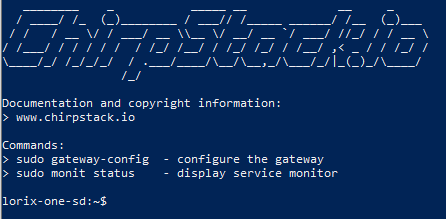
\includegraphics[width=\textwidth]{illustration/chirpstack_io_main_screen.PNG}}
  \caption{Interface layout of ChirpStack Gateway OS full, when the user has logged in}
  \label{fig:ChirpStack_gateway_os}
\end{figure}

As mentioned earlier the micro\gls{sd} card was provided with the ChirpStack \gls{os} and also with the needed credentials to log in.
The data the card contained the latest settings that Metropolia University of Applied Sciences uses and new configurations were not needed.
The command prompt was closed with an exit command.

\section{Creating Excel file for end devices}
The Excel file format was selected for storing the information about the application name and its details and all the devices that it should have in it.
The decision to utilize an Excel file was selected due to a accessibility of a pre-existing library called RPA.Excel.Files in Robot Framework.

\clearpage

The Excel file, \path{Applications.xlsx}, layout was designed so that each sheet the file includes would be named after the application name that the sheet contains.
When a sheet is opened it has three headers focusing on the application in the first row.
Those headers are called Application name, Application description and Service profile.
On the second row under each header of the columns the information is stored accordingly so that the data can be fetched by using the headers.

Row four contains headers for adding a \gls{lora} device to the application.
Those headers are called Device name, Device description, Device \gls{eui}, Device-profile and Application key.
Under those headers the user adds the device information correspondingly.

The Device \gls{eui} consists of 16 digits and/ or characters that can be given using three different forms, all written together, or with whitespaces, or colons as separators.
The parsing of colons and whitespaces is handled by ChirpStack.
The restrictions for the \gls{eui} code are that it can not include special characters in any form, as they are ignored by ChirpStack.
When the \gls{eui} is given to the corresponding field and a lack of correct amount of accepted digits and/ or characters, it results to an error when the device is tried to be added.

The Excel file filling is fully manual and left to the educator to fill in, but for this project three mock up sheets were created to test that the functionality works correctly.

\section{Creating automation}
This section will give an overview of how the automation was created for the project.
The automation was done using Robot Framework in the Visual Studio Code source code editor as it provides the possibility to implement Robot Framework and Robocorp extensions that were used.

The first step to start the automation was to build up the project structure for the ease of maintenance.
The project directory contains two main folders called automation and resources alongside with the \path{.gitignore} file and the \path{requirements.txt} file.
The automation folder contains the two robot files used for the automation, \path{__init__.robot} and \path{automation.robot}.
The resources folder is used in this project to store the \path{variables.py} file which is used in the project.
All the required packages and libraries are included in the \path{requirements.txt} file.

\subsection{variables.py}
The \path{Variables.py} is a python file where all the variables are stored to easily modify them if needed from one place.
The \path{variables.py} file includes a list of variables that are used in the suite setup and teardown, but also in the process automation.

All the variable names were created using uppercase characters and snake case in the naming to provide a better readability and recognition of the origin of the variables.
The variables used and crea\path{automation.robot} file were created with low case characters witted in the h the same snake case style.

A mockup version of the file is provided in Appendix~\ref{appx:sourcecode} to see what kind of formats were used.

\subsection{Suite Setup and Suite Teardown}

In this project Suite setup was selected to be utilized to eliminate unnecessary repetition of steps to be taken and to verify the pre-steps are functioning correctly before the tasks are run.
Suite setup was utilized in a suite initialization file called \path{__init__.robot} file which is run once and before files of the automation folder are executed.

The Suite Setup setting that was implemented is called Login to ChirpStack.
The task opens the browser with the browser type that was specified in the \path{variables.py} file.
For running the automation with a window where the user can see the progress while it runs, the headless argument was set to false.
When the browser is opened the next keyword takes the \gls{ip} address of the ChirpStack server for the login page that was initialized in the \path{variables.py} file.
The code then proceeds to fill the text fields for username and password also with values that were initialized in the \path{variables.py} file.
When the login credentials have been filled the task clicks the Login button.
Web elements, like the Login button, have been identified with selectors, mostly using the xpaths of those elements.
Some required a text identifier beside them to recognize them when an xpath is the same with another element.
The task then uses keywords to save the \gls{url} of the updated page to a variable and then compares it to the expected \gls{url}.
Lastly, the amount of items on a page of the applications list is set to be 100.

When the \path{automation.robot} file is executed the logs show if the setup passed alongside with the tasks.
If the suite setup fails the tasks will also be set to fail status\cite{robotFrameworkUserGuide:suiteSetupAndTeardown}.

The Suite Teardown setting is called Log out from ChirpStack.
The teardown navigates to the Logout button by pressing the username on the top right corner of the web interface and clicks the  Logout button.
The browser is then closed.

Suite teardown is executed after all test cases and child suites of a test suite are run.
It is always run no matter what the execution results of the test cases are or if the suite setup has failed.
If the teardown fails, all the tests of the test suite are set to fail status\cite{robotFrameworkUserGuide:suiteSetupAndTeardown}.

\subsection{Process automation}
The \path{automation.robot} file consists of tasks that were used for creating the application, adding and deleting devices and to delete a selected application.

The file has one task called main which executes a keyword named \textit{Take User Input}.
\textit{Take User Input} asks the user which of the named four tasks, seen in Figure~\ref{fig:user_input_commands}, is to be executed and after the selection the corresponding actions are made.
For utilizing these tasks four Robot Framework libraries were imported in the settings section: Browser, Dialogs, RPA.Excel.Files and Collections.

\clearpage

\begin{figure}[ht]
  \centering
  {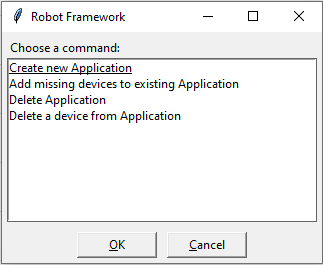
\includegraphics[width=10cm]{illustration/take_user_input_dialog.PNG}}
  \caption{Dialog pop-up window, where the user can select the task they want to be executed}
  \label{fig:user_input_commands}
\end{figure}

When \textit{Take User Input} is run, a list is acquired from the \textit{Get Application elements as lists} keyword.
The keyword goes through all the applications that are listed on the Applications layout of the ChirpStack Application server.
Each list item contains the ID, name, service-profile and description of the application.
The information of them is stored as elements in four separate lists by the header types.
Those four lists are then added to another list which is returned when the keyword is run.
The returned list is then used to access all the application name elements.
The elements are then used to access all the application names with a \textit{Get Application Names} keyword.

The \textit{Get Application Names} keyword takes a list of application name elements as an input and goes it through while saving each element in the corresponding application name in the Applications layout on ChirpStack.

After the application names are saved on a list a user input is asked to select what command is to be executed.
The commands are using the \textit{Get Selection From User} keyword of the Dialog library\cite{robotFramework:dialogsLibrary}, that shows a list of the named selection options in a pop-up window.
When that is selected the \textit{Take User Input} task proceeds to find the corresponding command name from an if--else statement and actions inside the statement are run after.
The following sections walk through all the commands and what their content consists of.


The Create Application command is the first one on the list of selections the user can take.
It saves all the existing worksheets from the \path{Applications.xlsx} file using the \textit{List worksheets on Excel} keyword of the RPA.Excel.Files library\cite{rpaFramework:excelFiles}.
After that \textit{Remove Already Existing Application Names from Sheet Options} is run with two list inputs, the list of Excel worksheets and another with the existing application names, which were obtained when the task begun to run.

\textit{Remove Already Existing Application Names from Sheet Options} goes through the application names from ChirpStack using a for-loop. The loop compares the current application name to the list of worksheet names from the Excel file and if a match is found, the application name is removed from the worksheet names.
This keyword is used to remove all the application names that already exist in the ChirpStack server from the list of options, from where the user can select the new application from.

The returned list from \textit{Remove Already Existing Application Names from Sheet options} is then inspected.
If the list size is zero, there are no new applications to add from the Excel file and a text input is added to the list and given as a selection to the user to exit the program.
If there are worksheet names left on the list instead, the program proceeds to provide another list of selections to user.
This pop-up window asks the user to select which application from the options the user wants to add and lets the user know of possibly removed options.
Figure~\ref{fig:new_application_select_application} provides screenshots of both dialog options mentioned above.
When the application name is selected the \textit{Create Application} keyword is run with the name as an input.

\clearpage

\begin{figure}[H]
  \centering
  \begin{tabular}{@{}c@{}}
    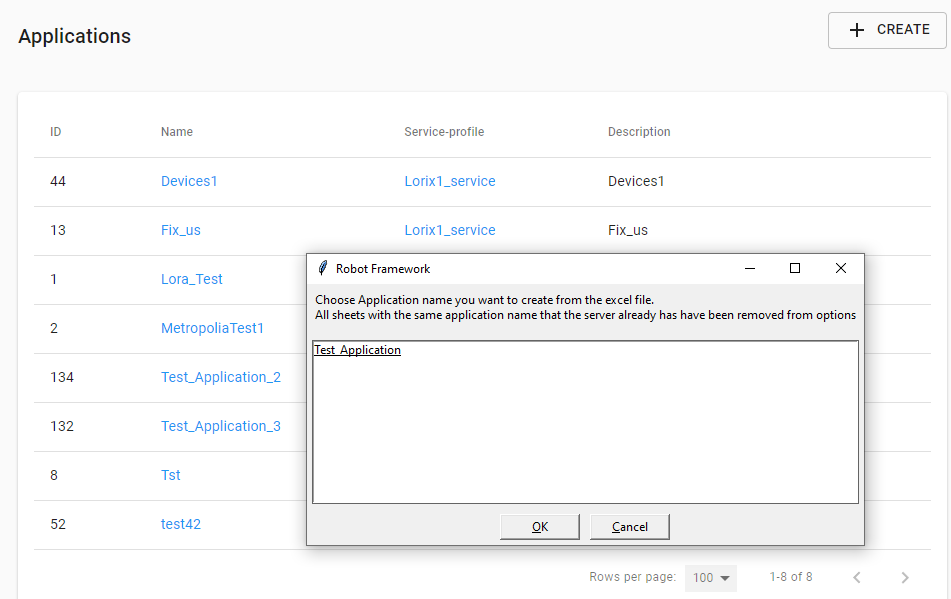
\includegraphics[width=\textwidth]{illustration/create_new_application_choose_application_dialog.PNG} \\[\abovecaptionskip]
    \small (A) Dialog pop-up window, where the user can select the application they want to create, \\ based on what applications from the Excel sheet are already added to the server
  \end{tabular}

  \vspace{\floatsep}

  \begin{tabular}{@{}c@{}}
    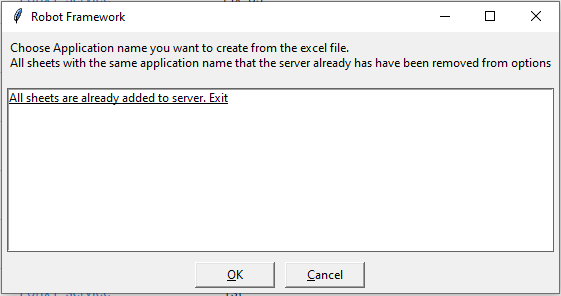
\includegraphics[width=12cm]{illustration/all_sheets_are_already_added.PNG} \\[\abovecaptionskip]
    \small (B) Dialog pop-up which is shown when all the applications from the Excel file are already added to \\ the ChirpStack server
  \end{tabular}

  \caption{Dialog pop-up is shown to the user when they select the Create Application command. Two variations of the content are available depending on what applications are already added from the Excel file.}\label{fig:new_application_select_application}
\end{figure}

\clearpage

\textit{Create Application} opens the worksheet of the \path{Applications.xlsx} file that has the given application name.
The name is verified to be there, as the list of selection was based on the worksheet names of this file.
First the Create button is clicked to access the create application layout.
The keyword then uses the keywords of the RPA.Excel.File library to save the worksheet as a table and to read the cell values from the second row of the worksheet, to access the application details which are added to the corresponding fields on the web interface.
When the new Application is created the layout changes to the list of all applications.
The keywords to access the application names are used to verify the newly created application is added and to access its name element.
The name element is then used with the \textit{Open Application} keyword to access the application and to add the devices from the worksheet.

The \textit{Add Devices} keyword is run from the opened layout of the  application.
It opens the Excel file from a worksheet with the same name as the application and saves the device information of all devices as a table.
The table is then gone through with a for-loop to use the \textit{Add One Device} keyword to save the devices one by one.
\textit{Add One Device} opens the device creation layout and fills in the required information to the web interface it has got from the Excel file.
If a device already exists, it means there is a device with the same name on the same application already, or a device with the same \gls{eui} is already added to the server.
If the problem lies with the two identical device names in the same application, the second one that is tried to be added is just ignored and the keyword returns.
If that is not the case, the keyword proceeds to use the \textit{Find a Device EUI from Application Names} keyword to find in which application it already exists on.
That application name is saved by the keyword and saved to the worksheet of the application from where the device was tried to be added.
This way the educator can easily see from the row of the device the device location on the server and remove it if needed.
If there was a problem adding the device \textit{Add One Device} returns to the application layout to proceed to add the rest of the application.
When all the devices are added the Create Application command is finished.

The second command in the Get Selection From User keyword of the \textit{Take User Input} task is called Add missing devices to existing Application.
This command lists all the applications that are already added to ChirpStack from the Excel file.
That list is then provided to the user using the same \textit{Get Selection From User} keyword from the Dialogs library \cite{robotFramework:dialogsLibrary} as mentioned earlier.
The selected application is then opened and the \textit{Add Devices} keyword is called.
\textit{Add Devices} is a suitable option for this command as well for its previously mentioned feature to ignore all the devices with an identical name on the selected application.

The third command in the \textit{Take User Input} is called Delete Application.
The command lists all the existing applications on the web interface for the user to select the one to delete, as seen in Figure~\ref{fig:delete_application}.

\begin{figure}[ht]
  \centering
  {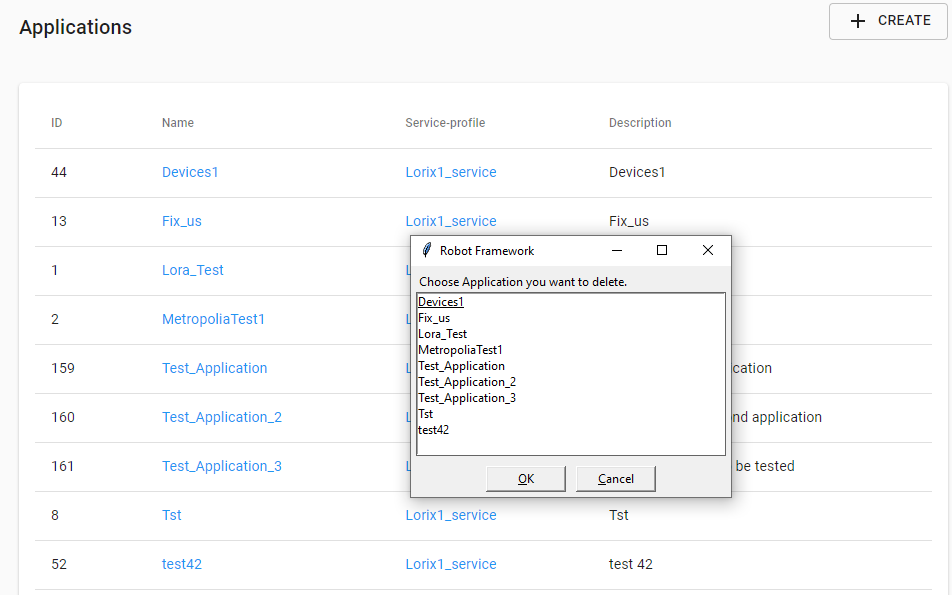
\includegraphics[width=\textwidth]{illustration/delete_app_choose_app_dialog_with_applications_on_back.PNG}}
  \caption{Dialog pop-up window, where the user can select the application they want to delete, based on what applications already exist on the server}
  \label{fig:delete_application}
\end{figure}

The last of the commands in \textit{Take User Input} is named Delete a device from Application.
It lists all the existing applications from the ChirpStack server for the user to make the selection, as seen in Figure~\ref{fig:delete_device_select_application}.

\clearpage

\begin{figure}[ht]
  \centering
  {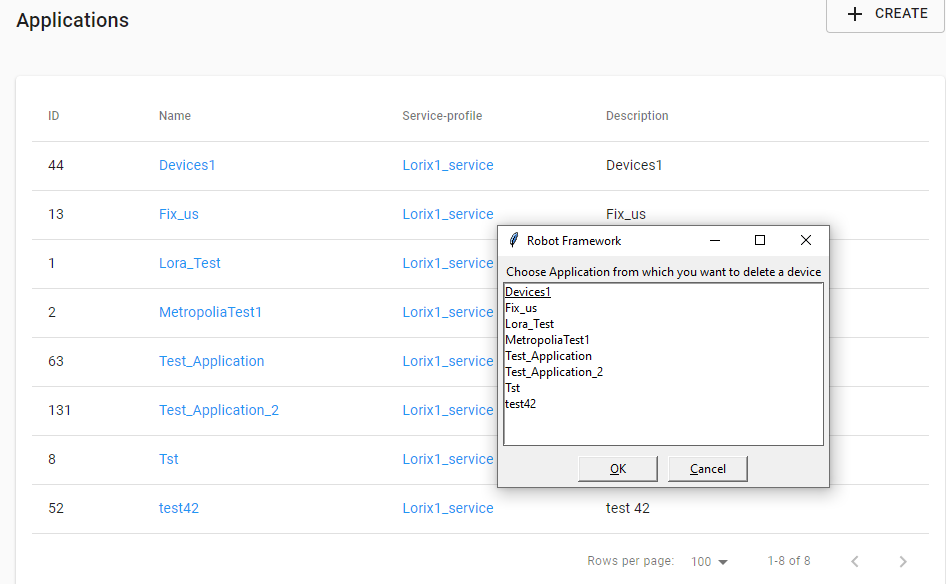
\includegraphics[width=\textwidth]{illustration/delete_device_choose_app_dialog_with_applications_on_back.PNG}}
  \caption{Dialog pop-up window, where the user can select the application they want to delete the device from, based on what applications already exist on the server}
  \label{fig:delete_device_select_application}
\end{figure}

After the application is selected, the command proceeds to list all the devices in a similar way, as seen in Figure~\ref{fig:delete_device_from_application_choose_device}.
If the application has no added devices, the command offers possibility to delete the application instead.

\begin{figure}
  \centering
  \begin{tabular}{@{}c@{}}
    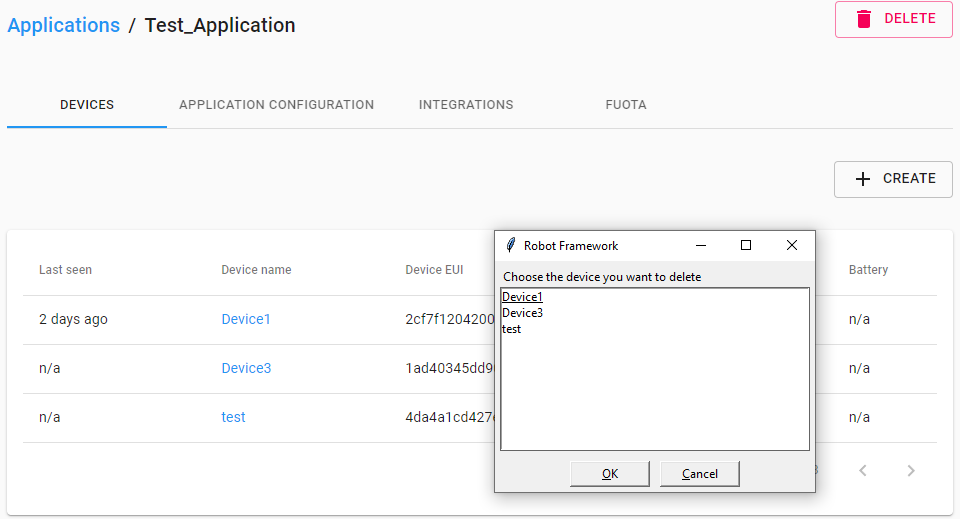
\includegraphics[width=\textwidth]{illustration/delete_device_from_app_choose_device_dialog_application_on_back.PNG} \\[\abovecaptionskip]
    \small (A) Dialog pop-up window, where the user can select the device they want to delete. \\ The list is based on what devices are added to the selected application on the server.
  \end{tabular}

  \vspace{\floatsep}

  \begin{tabular}{@{}c@{}}
    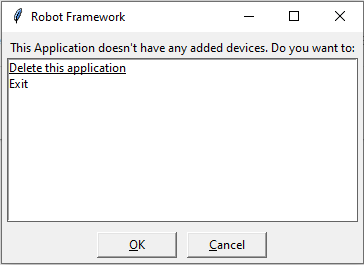
\includegraphics[width=10cm]{illustration/no_devices_to_delete.PNG} \\[\abovecaptionskip]
    \small (B) Dialog pop-up window, which is shown when there are no devices \\ to delete in the selected application.
  \end{tabular}

  \caption{Dialog pop-up window options, when the user selects the Delete a device from Application command. The window varies depending if there are any added devices on the chosen application.}\label{fig:delete_device_from_application_choose_device}
\end{figure}

\clearpage

\subsection{Testing}
When the implementation was done testing the functionality and comparing the efficiency could be done.
The functionality was tested by running the commands through with all the options used.
The \gls{lora} end device details were added to the Excel file and the devices were plugged to a power source to run the Python scripts to boot the devices.
Usually the students use one \gls{lora} module attached to a board, but to test more devices two modules were used in one board and two boards were provided for the testing purposes, so four devices in total were tested.
For this reason the Python script needed some modifications as it was implemented to boot one device only.
One of the updated scripts can be found from Appendix~\ref{appx:testing}.
The other one only has different application key defined to one of the devices, so one variable value is different.
After the devices were added to ChirpStack they could be manually accessed from the web interface.
From there the device details could be checked together with the data transmitting.
The devices were added to two of the three applications that were in the \path{Application.xlsx} file.
One of the devices had been defined with a different application key in both the Python script and the Excel file.
All the devices were successfully connected to ChirpStack and were transmitting data simultaneously as expected.

Efficiency was tested by running the Create Application command in different ways and by measuring the execution time.
This was done by creating three applications in each method, and the applications had a different amount of devices to see the differences in a longer run.
The first application had five devices, second 20, and third 45.
The first test run was done manually by using the Excel file details to copy paste them to Create the Application and to add all the devices.
Some devices are set to be faulty and the measuring also includes the time it took to process them as well.
The second run was done by running the implementation in windowed mode and the third also with the implementation, but with the headless mode.

\clearpage

Windowed and headless modes were quite close to each other in all the cases with all the scenarios, the headless mode being a few seconds faster in each test run.
Both of them outran the manual scenarios with their speed.
The longest run with the 45 device scenario took around 2.5 minutes with the headless and windowed mode, which took almost 19 minutes to perform manually.
Next, Chapter~\ref{ch:res_and_disc} shows plots of the testing results and Appendix~\ref{appx:tables} shows tables with the data that was gathered from testing and used in the plots.

\clearpage %force the next chapter to start on a new page. Keep that as the last line of your chapter!

% Results and discussion

\chapter{Results and Discussion} \label{ch:res_and_disc}

This chapter describes the obstacles and insights what have been faced during the implementation of the project and how the results came out to be.
It gives variations of what could have done differently and how the project can be improved in the future.
The chapter also discusses the pros and cons about the current maintainability.

\section{Results}
The implementation of this project offers a script that automates the process of adding new applications with new devices to a ChirpStacks server from an Excel file, with addition to add devices to an application that is already on the server and listed in the Excel file.
It also provides a possibility to delete single devices from the chosen application, as well as a possibility to delete an application with its devices from the server.

The implementation fulfills all of the requirements that were set in the beginning of the project with the additional request for a feature to delete an application by using its name.
The end result provides the user a way to handle the tasks more effectively than previously by reducing the possible human errors in writing and by speeding up the process.
As the implementation can be executed repeatedly, when the settings and other factors are still the same, it can potentially save a lot of time from the educators.

The implementation's effectiveness has been tested by comparing the workload of adding a new application with a set of devices to the server either manually or by using the implementation.
The testing also took in consideration about the difference if the browser is run headless or with the visible window.
The manual part was implemented by using the same Excel file where the details where added, and that was applied by writing all the details fully manually and by using the copy-paste method to speed things up a bit.
The test is only done by one person, therefore the writing speed is a changing factor and the time measuring is not as specific, as it would be if the time would be measured by an other person, or a computer.

Below there are three plots shown. Each one represents one test case. First one is to create an application with 5 devices in Figure\ref{fig:5_devices}, second with 20 devices in Figure\ref{fig:20_devices} and third with 45 devices in Figure\ref{fig:45_devices}.
The time that has been used to select the command to create the application and then the wanted application is excluded from the time measurements.

Each plot shows the amount of time it has taken to add the devices to the application by executing it in three different ways, manually, using the windowed mode and the headless mode of the implementation.
Time is an increasing curve showing the total amount used in the process of adding the devices.
Three tables are attached to Appendix~\ref{appx:tables}to show the amount of time to create application in the same three methods that are used in the plotting.

\begin{figure}[H]
\centering
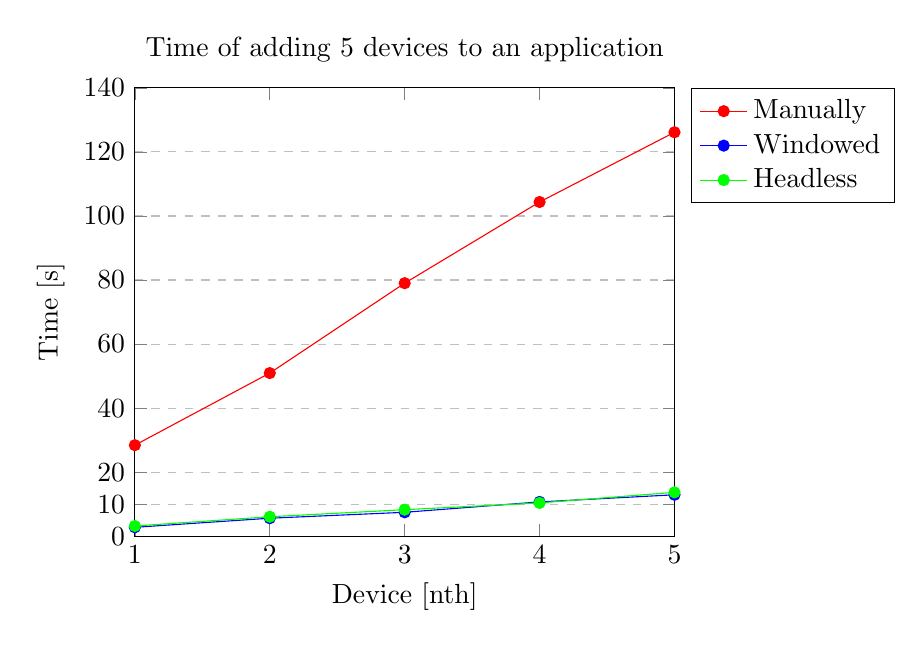
\begin{tikzpicture}
\begin{axis}[
    title={Time of adding 5 devices to an application},
    xlabel={Device [nth]},
    ylabel={Time [s]},
    xmin=1, xmax=5,
    ymin=0, ymax=140,
    xtick={1,2,3,4,5},
    ytick={0,10,20,40,60,80,100,120,140},
    legend pos=outer north east,
    legend cell align=left,
    ymajorgrids=true,
    grid style=dashed,
]

\addplot[
    color=red,
    mark=*,
    ]
    coordinates {
    (1,28.42)
    (2,50.94)
    (3,79.01)
    (4,104.36)
    (5,126.14)
    };
\addplot[
    color=blue,
    mark=*,
    ]
    coordinates{
    (1,2.776)
    (2,5.616)
    (3,7.463)
    (4,10.706)
    (5,12.929)
    };
\addplot[
    color=green,
    mark=*,
    ]
    coordinates{
    (1,3.176)
    (2,6.074)
    (3,8.274)
    (4,10.391)
    (5,13.692)
    };
    \legend{Manually, Windowed, Headless}
\end{axis}
\end{tikzpicture}

    \caption{Plot represents the results of testing the efficiency to add 5 devices to an application with three execution modes: manual, automated windowed mode and automated headless mode. Corresponding table to show data for each coordinate value is found from Table~\ref{tab:5_devices}}\label{fig:5_devices}
\end{figure}

\begin{figure}[H]
\centering
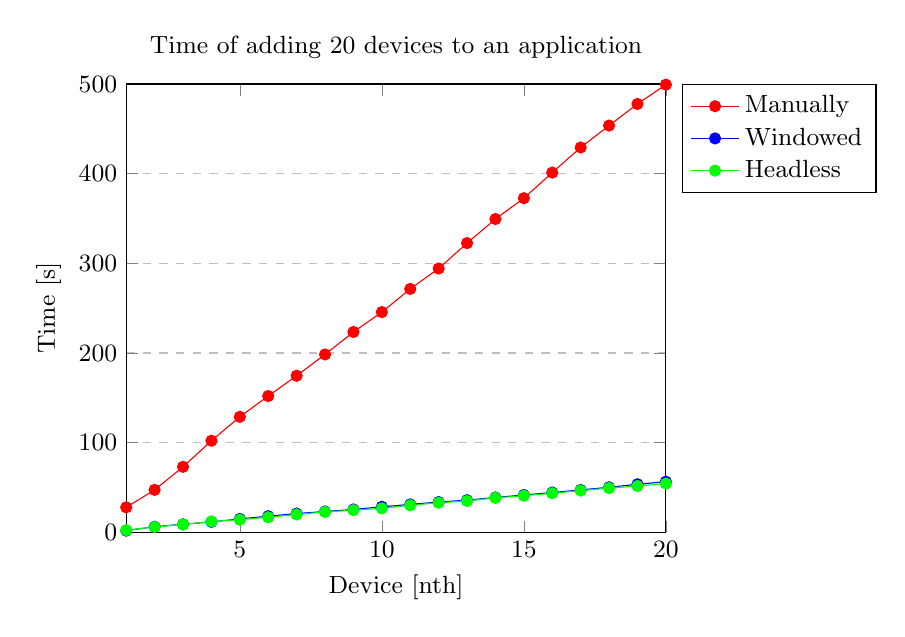
\begin{tikzpicture}
\begin{axis}[
    title={Time of adding 20 devices to an application},
    xlabel={Device [nth]},
    ylabel={Time [s]},
    xmin=1, xmax=20,
    ymin=0, ymax=500,
    xtick={0,5,10,15,20},
    ytick={0,100,200,300,400,500},
    legend pos=outer north east,
    legend cell align=left,
    ymajorgrids=true,
    grid style=dashed,
]

\addplot[
    color=red,
    mark=*,
    ]
    coordinates {
    (1,27.88)
    (2,47.36)
    (3,73.07)
    (4,102.17)
    (5,128.83)
    (6,152.03)
    (7,174.65)
    (8,198.41)
    (9,223.45)
    (10,245.63)
    (11,271.48)
    (12,294.25)
    (13,322.59)
    (14,349.44)
    (15,372.66)
    (16,401.25)
    (17,429.23)
    (18,453.67)
    (19,477.78)
    (20,499.28)
    };
\addplot[
    color=blue,
    mark=*,
    ]
    coordinates {
    (1,1.889)
    (2,6.244)
    (3,8.979)
    (4,11.591)
    (5,14.987)
    (6,18.008)
    (7,20.925)
    (8,23.241)
    (9,25.504)
    (10,28.466)
    (11,31.14)
    (12,33.822)
    (13,35.882)
    (14,38.861)
    (15,41.661)
    (16,44.417)
    (17,47.286)
    (18,50.244)
    (19,53.619)
    (20,56.474)
    };
\addplot[
    color=green,
    mark=*,
    ]
    coordinates {
    (1,2.413)
    (2,6.028)
    (3,8.763)
    (4,12.080)
    (5,14.112)
    (6,16.761)
    (7,19.961)
    (8,22.730)
    (9,24.710)
    (10,26.742)
    (11,30.158)
    (12,33.057)
    (13,35.023)
    (14,38.424)
    (15,40.858)
    (16,43.574)
    (17,46.574)
    (18,49.372)
    (19,51.672)
    (20,54.404)
    };
    \legend{Manually, Windowed, Headless}
    \small Plot showing the amount of time to add 20 devices.
\end{axis}
\end{tikzpicture}

    \caption{Plot represents the results of testing the efficiency to add 20 devices to an application with three execution modes: manual, automated windowed mode and automated headless mode.Corresponding table to show data for each coordinate value is found from Table~\ref{tab:20_devices}}\label{fig:20_devices}
\end{figure}

\begin{figure}[H]
\centering
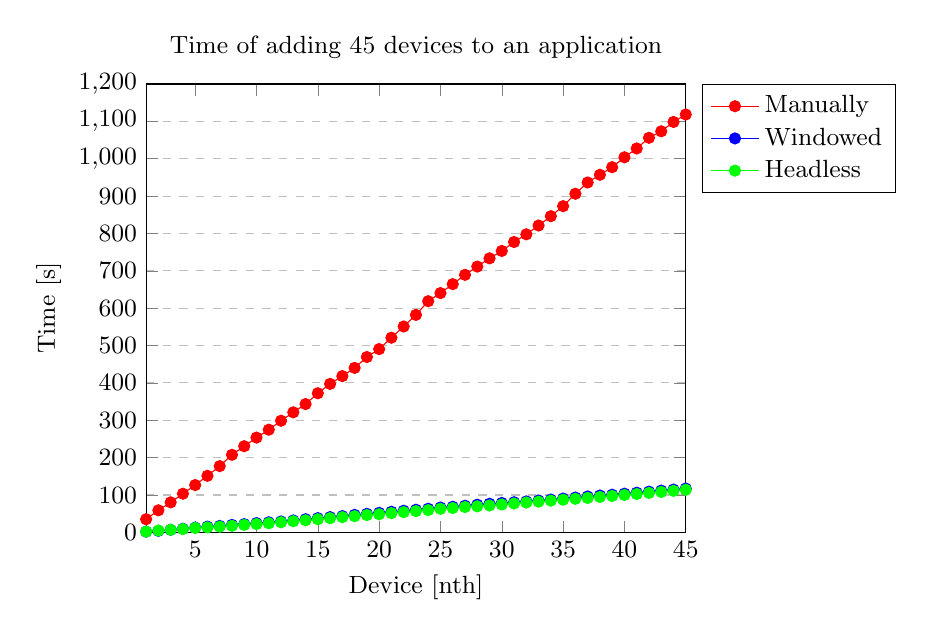
\begin{tikzpicture}
\begin{axis}[
    title={Time of adding 45 devices to an application},
    xlabel={Device [nth]},
    ylabel={Time [s]},
    xmin=1, xmax=45,
    ymin=0, ymax=1200,
    xtick={0,5,10,15,20,25,30,35,40,45},
    ytick={0,100,200,300,400,500,600,700,800,900,1000,1100,1200},
    legend pos=outer north east,
    legend cell align=left,
    ymajorgrids=true,
    grid style=dashed,
]

\addplot[
    color=red,
    mark=*,
    ]
    coordinates {
    (1,35.15)
    (2,59.01)
    (3,80.32)
    (4,103.42)
    (5,126.60)
    (6,151.33)
    (7,177.22)
    (8,207.59)
    (9,230.60)
    (10,253.61)
    (11,274.75)
    (12,298.70)
    (13,321.28)
    (14,343.35)
    (15,372.32)
    (16,397.39)
    (17,418.24)
    (18,440.21)
    (19,469.28)
    (20,490.53)
    (21,521.04)
    (22,551.04)
    (23,582.11)
    (24,618.71)
    (25,640.46)
    (26,664.43)
    (27,689.26)
    (28,711.40)
    (29,733.45)
    (30,753.23)
    (31,777.15)
    (32,797.72)
    (33,821.30)
    (34,846.26)
    (35,873.10)
    (36,906.32)
    (37,936.40)
    (38,957.09)
    (39,977.44)
    (40,1003.96)
    (41,1027.56)
    (42,1056.00)
    (43,1073.48)
    (44,1098.45)
    (45,1118.44)
    };
\addplot[
    color=blue,
    mark=*,
    ]
    coordinates {
    (1,1.915)
    (2,4.041)
    (3,6.777)
    (4,9.584)
    (5,12.646)
    (6,15.298)
    (7,17.269)
    (8,19.895)
    (9,21.986)
    (10,24.673)
    (11,26.902)
    (12,29.104)
    (13,31.922)
    (14,35.189)
    (15,37.995)
    (16,40.729)
    (17,43.367)
    (18,46.807)
    (19,49.507)
    (20,52.167)
    (21,55.02)
    (22,57.709)
    (23,60.466)
    (24,63.079)
    (25,66.391)
    (26,68.453)
    (27,71.064)
    (28,73.917)
    (29,76.447)
    (30,78.653)
    (31,80.53)
    (32,82.813)
    (33,85.196)
    (34,87.703)
    (35,90.392)
    (36,93.141)
    (37,96.044)
    (38,98.565)
    (39,100.655)
    (40,103.475)
    (41,106.123)
    (42,108.887)
    (43,111.672)
    (44,114.399)
    (45,117.309)
    };
\addplot[
    color=green,
    mark=*,
    ]
    coordinates {
    (1,1.954)
    (2,4.799)
    (3,6.93)
    (4,8.948)
    (5,11.764)
    (6,13.348)
    (7,15.314)
    (8,17.514)
    (9,19.999)
    (10,22.13)
    (11,24.297)
    (12,26.963)
    (13,29.763)
    (14,32.296)
    (15,35.081)
    (16,37.829)
    (17,40.613)
    (18,43.279)
    (19,46.279)
    (20,48.477)
    (21,51.327)
    (22,54.111)
    (23,56.759)
    (24,59.424)
    (25,63.008)
    (26,65.024)
    (27,67.758)
    (28,69.624)
    (29,71.956)
    (30,74.589)
    (31,77.189)
    (32,79.888)
    (33,82.121)
    (34,84.853)
    (35,87.352)
    (36,89.786)
    (37,92.118)
    (38,94.701)
    (39,97.401)
    (40,99.932)
    (41,102.536)
    (42,105.499)
    (43,108.149)
    (44,111.165)
    (45,113.998)};
    \legend{Manually, Windowed, Headless}
    \small Plot showing the amount of time to add 45 devices.
\end{axis}
\end{tikzpicture}
    \caption{Plot represents the results of testing the efficiency to add 45 devices to an application with three execution modes: manual, automated windowed mode and automated headless mode.Corresponding table to show data for each coordinate value is found from Table~\ref{tab:45_devices}}\label{fig:45_devices}
\end{figure}

\clearpage

\section{Faced difficulties}
The challenges that were faced during the project consisted of different kind of problems.
The most common ones would be trying to find errors that were faced during the testing of the features.
Most difficult ones to spot relating to that turned out to be the ones where syntax errors were occurring in the Robot Framework script, and incorrect amount of whitespace in different keywords.

The Lorix One gateway also provided some extra obstacles.
During testing, the web-interface started to refuse the connection and testing needed to be paused.
In the beginning this was handled by rebooting the server and it fixed the problem.
The reason for this was not found.

Later on there was a new problem, when the feature of deleting a selected device from the decided application was being tested.
This feature had functioned correctly earlier and no changes were made to the Robot Framework script. 
The problem was noticed when the gateway had been rebooted and the testing was continued for that feature.
The problem was that when a device is being deleted from an application, after clicking the delete button the user is to be expecting a confirmation message.
Instead the server showed a pop-up error message on the bottom left page as seen in Figure~\ref{fig:error_when_confirming_device_deleting}.

\begin{figure}[ht]
  \centering
  {
\includegraphics[width=\textwidth]{illustration/error_when_confirming_device_deleting.PNG}}
  \caption{Error message about refused connection to the Redis server that is run by the ChirpStack \gls{os}}
  \label{fig:error_when_confirming_device_deleting}
\end{figure}

Further investigation through ChirpStack forum resulted to find people with similar problem when using the same gateway \cite{chirpstack_forum:redis_error}.
Later on in the discussion, a user proposed a possible solution that can be found in an opened issue on GitHub \cite{github:redis_issue}.
A collaborator in the GitHub project had made changes to the \path{redis.conf} file in the ChirpStack \gls{os} to fix the issue.
That same fix was used in this project to outrun the problem and it got solved.

During the last few test runs the connection to the web-interface was corrupted again, the issue being that while the user got logged in, no applications were visible in the server and therefor they were not accessible either.
The first hand solution, that worked, was to disconnect the gateway for overnight and turn it on again.
After that the issue never came back, so there was no further investigation.

Overall these server obstacles slowed down the project implementation with several days.
Further investigation should be considered if the problems continue.
This might require to take some actions, like updating the software versions, or even to change the hardware that is used, as most of the challenges were reflected to the use of the Lorix One gateway.
The consideration should also take in account the load the gateway has been under during the testing.
The implementation is most likely not used as heavily in such short-term , as it has during the testing phases.


\section{Maintainability}
 Upon the beginning of the project it was decided that the automation was to be implemented by using Robot Framework.
 The hardware was decided to be the same that Metropolia University of Applied Sciences already use and it was delivered by them.

The implementation relies completely on the web-interface of the ChirpStack Application server.
The variables are created by using the selectors of the elements in the web-interface and they are hard-coded to the variables.py file.
If any changes to the web-interface is made, it might lead to breaking the Robot Framework script, or at least to a large amount of redefinition of the variables and possibly the keywords as well.

The Lorix One gateway only supports the ChirpStack up to the version 3, and all the implementation is also based to that version.
The most latest version of the ChirpStack is currently version 4.
If the gateway hardware, or the ChirpStack version is to be updated, it might make the implementation incompatible.

\section{Improvement ideas}

The implementation is currently made with the assumption that there is less than 100 applications listed, meaning they would be visible on a single page when the rows per page selection is set to 100.
And same default base is also used with the devices that are added to a single application.
If the amount of those applications or devices is greater than 100, the ones that are crossing the limit are shown in the next page,  and therefore aren't processed as part of the list.
Currently the rows per page amount is set in the suite setup and the selected row amount is automatically set to it in every list type in the web-interface.
This should be changed in the next possible update to make the implementation more reliable.

The Robot Framework script's running time, when multiple devices are added, could possibly be further reduced by handling all the message pop-ups that the device creation triggers.
Currently it verifies that there is no message about duplicate device, but on a successful device creation there is a device created message as well. 
This message leads to extra waiting time as the script recognizes it to one of the pop-ups and starts the timeout which delays the running time.
This issue could be solved for example by closing the device created pop-up, whenever it is triggered.

Robocorp announced the joining to Sema4.ai on the end of January \cite{robocorp:sema4.ai}.
In the following month they published that they are focusing to develop the automation further only in Python language.
The implementation is currently using RPA Framework's Excel.Files library to interact with the Excel files, using Robot Framework.
The new direction Robocorp is taking with the code focused automation means that the existing Robot Framework based libraries are being spared, but no new updates or issue fixes are done in regards to them.
In practise this affects the upcoming development, which should be considered if this project is to be further developed.

During the research about the ChirpStack Application server, it was found out that ChirpStack provides \gls{grpc} and \gls{rest}ful APIs \cite{chirpstack:applicationServer}.
ChirpStack stood down from using \gls{rest} API from the version 4 onwards.
With this in mind, it should be considered if the script is to be updated, that if it should be implemented by using the API provided with the \gls{grpc} instead of the current automation of the web-interface.
This would provide a list of more reliable commands to use for handling the tasks in the server.

\clearpage

Using the \gls{grpc} framework requires a decision about what programming language to use with it.
The \gls{grpc} officially supports 10 different languages, like C++, Python, Java, and Node.js to name a few examples, but there are also some community-based implementations available.

Even if the implementation would start to use \gls{grpc}, Robot Framework can still be the framework to be used.
Robot Framework supports extending through Python libraries and ChirpStack also supplies a Python \gls{sdk} for the \gls{grpc}.
With these complabilities in mind, Python could be considered as a strong candidate from the programming language options to use with the \gls{grpc}.



\clearpage %force the next chapter to start on a new page. Keep that as the last line of your chapter!
% Conclusions

\chapter{Conclusions} \label{ch:conc}

Check Final Year Project Guide for the content of Conclusions chapter.

\clearpage %force the next chapter to start on a new page. Keep that as the last line of your chapter!


% Sample content to demonstrate LaTeX command. You will likely delete this line and the 
% next \input{sample/*} lines. You are also safe to delete the sample/ folder and its
% content once you refershed your LaTeX skills. Also check the appendix samples.
%%sample content to demonstrate LaTeX command.

\chapter{Material and Methods}

This is a chapter to demonstrate some of the \LaTeX{} ~commands that you can use to format your text.
This should be \textbf{bold} and this \textit{italic} and finally \textbf{\textit{bolditalic}}. When one want to use an abbreviation or acronym like \gls{html} using the \textbf{\textbackslash{}gls} command in \gls{latex}, the first time, it comes with it full version and for all next uses in it short \gls{html} form. Of course, when needed, the full version is available using e.g. the \textbf{\textbackslash{}acrlong} command.

The defined terms like \gls{maths} use the same \textbf{\textbackslash{}gls} \gls{latex} command. The Capitalized can be obtained with \textbf{\textbackslash{}Gls}. Should be avoided; but to have all the abbreviations and terms, even the non-used ones, use the \textbf{\textbackslash{}glsaddall} command before printing the list of Abbreviations. 

\section{Section with references}
Here is an example how to cite a bibliography entry \cite{kopka:guide} using the \textquotedblleft\textbackslash{}cite\textquotedblright ~\gls{latex} command ~\cite[section 4.2]{tobias:book}. Note that a paragraph is added by forcing a new line.

And let also try the figure (see figure \vref{fig:latex-cover}) and internal reference (with label and ref or vref). The reference can be done to any label, for example why not to appendix \ref{appx:first} or to appendix \ref{appx:second}? To note, \gls{latex} will place the figure to the best place (except with forcing). Let them float till the final of final edit\ldots ~then force them to not break a paragraph.%hugly hack... I'm sorry
\begin{figure}[h]
  \centering
  
\includegraphics[width=7.1cm]{LaTeX_cover}
  \caption{\gls{latex} cover image (Copied from wikibooks.org (2012) \cite{wikibooks:latex}).}
  \label{fig:latex-cover}
\end{figure}

Let's also try a long quote:
From the Universal Declaration of Human Rights:
\begin{quote}
(1) Everyone has the right to education. Education shall be free, at least in the elementary and fundamental stages. Elementary education shall be compulsory. Technical and professional education shall be made generally available and higher education shall be equally accessible to all on the basis of merit.

(2) Education shall be directed to the full development of the human personality and to the strengthening of respect for human rights and fundamental freedoms. It shall promote understanding, tolerance and friendship among all nations, racial or religious groups, and shall further the activities of the United Nations for the maintenance of peace.

(3) Parents have a prior right to choose the kind of education that shall be given to their children. \cite[article 26]{un:udhr}
\end{quote}

\textit{Quisque augue} est, \textbf{elementum ac porttitor} non, porttitor ac orci. Donec hendrerit, ligula ac luctus egestas, sem dolor pretium nunc, sed vehicula magna diam a massa. Donec mattis, arcu et tempor mattis, risus tortor ultrices metus, nec sodales sem dolor eu elit.\vspace{-17pt} 
\begin{itemize}
\item \textbf{A small hack} with list
\item is to force the vertical space 
\item before and after the list
\end{itemize}
\vspace{-17pt} Nullam egestas enim at odio pellentesque bibendum. 

\subsection{Subsection}
Donec et sapien ac leo condimentum vulputate id et tellus. Maecenas hendrerit malesuada interdum. Aenean dignissim sem faucibus elit congue faucibus id non risus. Morbi at dui non tortor pellentesque consequat non eget urna. Cras in sapien dui, a tincidunt velit.
\reaction{\label{eq:reaktio}$\underset{\text{+II}}{\ce{2Fe^2+}}$ + $\underset{\text{+I\;-I}}{\ce{H2O2}}$ + $\underset{\text{+I\;-II}}{\ce{2H3O^+}}$ <=> $\underset{\text{+III}}{\ce{2Fe^3+}}$ + $\underset{\text{+I\;-II}}{\ce{4H2O}}$}
Työn aluksi rauta(II)ionit hapetetaan rauta(III)ioneiksi väkevällä vetyperoksidilla, kuten reaktion~\ref{eq:reaktio} hapetusluvuista nähdään (rauta hapettuu, happi pelkistyy).  
\reaction{Fe^3+( \emph{aq} ) + 3OH^-( \emph{aq} ) + $(x-1)$H2O( \emph{l} ) -> FeOOH $\cdot$ $x$(H2O)( \emph{s} )}
Rauta(III)ionit saostetaan emäksen (\ce{NH3}) avulla ja saadaan tuotteeksi kidevedellinen rauta(III)hydroksidi. Saatu saostuma pestään \ce{NH4NO3}:lla.
\reaction{FeOOH $\cdot$ $x$(H2O)( \emph{s} ) ->T[$\Delta$900-1000\celsius] Fe2O3( \emph{s} )}

\subsection{Subsection with \Gls{maths}}
Donec et sapien ac leo condimentum vulputate id et tellus. Maecenas hendrerit malesuada interdum. Aenean dignissim sem faucibus elit congue faucibus id non risus. Morbi at dui non tortor pellentesque consequat non eget urna. Cras in sapien dui, a tincidunt velit. Tertiäärinen butyylikloridi reagoi veden kanssa oheisen reaktion mukaisesti:
\reaction{(CH3)3CCl + 2H2O -> (CH3)3COH+H3O+ +Cl-}
Kyseessä on ensimmäisen kertaluvun reaktio, joten reaktion nopeus on
\begin{align}
v=-\frac{\mathrm{d}[\tn{t-ButCl}]}{\mathrm{d}t}=\frac{\mathrm{d}[\tn{HCl}]}{\mathrm{d}t}=k[\tn{t-ButCl}]
\end{align}
Jos tarkastellaan lähtöaineen t-butyylikloridin häviämistä saadaan
\begin{align}
\frac{\mathrm{d}[\tn{t-ButCl}]}{[\tn{t-ButCl}]}&=-k\mathrm{d}t \\
\int \frac{\mathrm{d}[\tn{t-ButCl}]}{[\tn{t-ButCl}]}&=-k \int \mathrm{d}t \\
\ln \int_{[\tn{t-ButCl}]_0}^{[\tn{t-ButCl}]} [\tn{t-ButCl}]&=-k\int_0^t t \\
\ln \left( \frac{[\tn{t-ButCl}]}{[\tn{t-ButCl}]_0} \right)&=-kt
\end{align}
Ionivahvuus lasketaan kaavalla.
\begin{align}
I&=\frac{1}{2}\cdot\sum z_i^2c_i \\
z_i&= \tn{ionin varausluku} \\
c_i&= \tn{ionin konsentraatio}
\end{align}
Aktiivisuuskerroin $\gamma_\pm$ lasketaan kaavalla.
\begin{align}
\log \gamma_\pm &= -\left|z_+\cdot z_-\right|A\cdot I^{\frac{1}{2}} \\
A &= \tn{0,509 (lämpötilassa 25\celsius}) \\
I &= \tn{ionivahvuus} \\
z &= \tn{ionien varaus}
\end{align}

\section{Section with Source Code}
Donec et sapien ac leo condimentum vulputate id et tellus. Maecenas hendrerit malesuada interdum. Aenean dignissim sem faucibus elit congue faucibus id non risus. Morbi at dui non tortor pellentesque consequat non eget urna. Cras in sapien dui, a tincidunt velit.

%For sharelatex users, use space instead of tab to avoid ^^I
\begin{code}
  \begin{minted}{php}
<?php
$userName = $_POST["usern"];
//maybe not?
if ($userName){
	?>
	<h2>Hello <?php echo $userName; ?>!</h2>
	<p>your message got received.</p>
	<?php
}
?>
\end{minted}
  \captionof{listing}{Descriptive Caption Text (e.g. this code do blah)}
  \label{code:testphp}
\end{code}


As see in listing \ref{code:testphp}, blah. It is also possible to have code inline, for example \mintinline{sql}{SELECT * FROM user WHERE age >= 18} that was SQL. 
The lisings \ref{code:htmlfull} and \ref{code:htmlpart} show how to load code from an external source file. In the case of listing \ref{code:htmlpart} it only take few line out of the source code file.

\begin{code}
  \inputminted{html}{code/html5_sample.html}
  \captionof{listing}{Some html code}
  \label{code:htmlfull}
\end{code}
 Donec et sapien ac leo condimentum vulputate id et tellus. Maecenas hendrerit malesuada interdum. Aenean dignissim sem faucibus elit congue faucibus id non risus.
 
 \begin{code}
   \inputminted[firstline=3,lastline=6]{html}{code/html5_sample.html}
  \captionof{listing}{The \mintinline{html}{<head>} section of an html page}
  \label{code:htmlpart}
\end{code}


 Morbi at dui non tortor pellentesque consequat non eget urna. Cras in sapien dui, a tincidunt velit.


\section{Section with Table}
Donec et sapien ac leo condimentum vulputate id et tellus. Maecenas hendrerit malesuada interdum. Aenean dignissim sem faucibus elit congue faucibus id non risus. Morbi at dui non tortor pellentesque consequat non eget urna. Cras in sapien dui, a tincidunt velit.

\begin{table}[h]
  \centering
  \caption{Some data}
  %IMPORTANT the caption must be before the tabular, so it will be on top of the table (there are other tricks to force it on top; but this one is straitforward).
  \begin{tabular}{| l | >{\centering\arraybackslash}p{.5\textwidth} |}
    \hline
    Test 1 & test 1234 test \\
    \hline
    Some more date comes here & with more values and if the text is very long it will disappear out of the box unless you force the column size :( \\
    \hline
  \end{tabular}
  \label{table:some_data}
\end{table}


As presented in table \ref{table:some_data}: Donec et sapien ac leo condimentum vulputate id et tellus. Maecenas hendrerit malesuada interdum. Aenean dignissim sem faucibus elit congue faucibus id non risus. Morbi at dui non tortor pellentesque consequat non eget urna. Cras in sapien dui, a tincidunt velit.

\begin{table}[h]
  \centering
  \caption{Another table with tabularx}
  \begin{tabularx}{.95\textwidth}{| l | >{\centering\arraybackslash} X |}
    \hline
    Test 1 & test 1234 test \\
    \hline
    Some more date comes here & with more values and if the text is very long it will disappear out of the box unless you force the table size :( \\
    \hline
  \end{tabularx}
  \label{table:some_data2}
\end{table}

As presented in table \ref{table:some_data2}: Donec et sapien ac leo condimentum vulputate id et tellus. Maecenas hendrerit malesuada interdum. Aenean dignissim sem faucibus elit congue faucibus id non risus. Morbi at dui non tortor pellentesque consequat non eget urna. Cras in sapien dui, a tincidunt velit.

\begin{table}[htbp]
  \centering
  \caption{Booktabs example}
    \begin{tabular}{rrrr}
    \toprule
    t (s) & [HCl] & [t-ButCl] & $\ln\frac{[t-ButCl]}{[t-ButCl]_0}$ \\
    \midrule
    0     & 4,02  & 160,88 & 0,00 \\
    10    & 63    & 101,9 & -0,46 \\
    20    & 115,2 & 49,7  & -1,17 \\
    30    & 141,3 & 23,6  & -1,92 \\
    40    & 157,9 & 7     & -3,13 \\
    50    & 161   & 3,9   & -3,72 \\
    60    & 164,3 & 0,6   & -5,59 \\
    70    & 163,5 & 1,4   & -4,74 \\
    80    & 163,8 & 1,1   & -4,99 \\
    90    & 164,1 & 0,8   & -5,30 \\
    100   & 164,3 & 0,6   & -5,59 \\
    \bottomrule
    \end{tabular}
  \label{tab:thisislabel}
\end{table}

As presented in table \ref{tab:thisislabel}: Donec et sapien ac leo condimentum vulputate id et tellus. Maecenas hendrerit malesuada interdum. Aenean dignissim sem faucibus elit congue faucibus id non risus. Morbi at dui non tortor pellentesque consequat non eget urna. Cras in sapien dui, a tincidunt velit.

\clearpage %force the next chapter to start on a new page. Keep that as the last line of your chapter!

%%Dummy content to use some space...

\chapter{Theory}

Lorem ipsum dolor sit amet, consectetur adipiscing elit. Aliquam aliquam aliquam purus, in ornare nulla imperdiet molestie. Nam tempus erat eu dui rhoncus et vestibulum mi elementum. Ut porttitor elit sit amet justo dignissim sit amet sagittis massa egestas. Mauris sed dolor eget dui fermentum sodales ut eu nibh. 

Quisque augue est, elementum ac porttitor non, porttitor ac orci. Donec hendrerit, ligula ac luctus egestas, sem dolor pretium nunc, sed vehicula magna diam a massa. Donec mattis, arcu et tempor mattis, risus tortor ultrices metus, nec sodales sem dolor eu elit. Nullam egestas enim at odio pellentesque bibendum. 

Donec et sapien ac leo condimentum vulputate id et tellus. Maecenas hendrerit malesuada interdum. Aenean dignissim sem faucibus elit congue faucibus id non risus. Morbi at dui non tortor pellentesque consequat non eget urna. Cras in sapien dui, a tincidunt velit.

\clearpage %force the next chapter to start on a new page. Keep that as the last line of your chapter!

%% Sample content to demonstrate tikzpicture

\chapter{Current State Analysis}

Data to plot the graph \ref{fig:stdplot} are in data.dat file.
Lorem ipsum dolor sit amet, consectetur adipiscing elit. Aliquam aliquam aliquam purus, in ornare nulla imperdiet molestie. Nam tempus erat eu dui rhoncus et vestibulum mi elementum. Ut porttitor elit sit amet justo dignissim sit amet sagittis massa egestas. Mauris sed dolor eget dui fermentum sodales ut eu nibh.
\begin{figure}[htbp]
  \centering
    \begin{tikzpicture}
        \pgfplotsset{width=12cm,
        compat=1.3,
        legend style={font=\footnotesize}}
    \begin{axis}[
    xlabel={c (mg/l)},
    ylabel={A},
    legend pos=north west,
    ymajorgrids=true,
    grid style=dashed
]

\addplot [only marks, blue] table {data.dat};
\addplot [no markers, thick, red] table[
x=c,
y={create col/linear regression}] {data.dat};
\addlegendentry{data}
\addlegendentry{%
$\pgfmathprintnumber{\pgfplotstableregressiona}x
\pgfmathprintnumber[print sign]{\pgfplotstableregressionb}$}
\end{axis}
\end{tikzpicture}
\caption{Simple linear regression plot (cannot get $r^2$ value)}
\label{fig:stdplot}
\end{figure}

Quisque augue est, as seen in figure \ref{fig:stdplot} elementum ac porttitor non, porttitor ac orci. Donec hendrerit, ligula ac luctus egestas, sem dolor pretium nunc, sed vehicula magna diam a massa. Donec mattis, arcu et tempor mattis, risus tortor ultrices metus, nec sodales sem dolor eu elit. Nullam egestas enim at odio pellentesque bibendum. 

Donec et sapien ac leo condimentum vulputate id et tellus. Maecenas hendrerit malesuada interdum. Aenean dignissim sem faucibus elit congue faucibus id non risus. Morbi at dui non tortor pellentesque consequat non eget urna. Cras in sapien dui, a tincidunt velit.

\section{Section}

Lorem ipsum dolor sit amet, consectetur adipiscing elit. Aliquam aliquam aliquam purus, in ornare nulla imperdiet molestie. Nam tempus erat eu dui rhoncus et vestibulum mi elementum. 
\tikzstyle{palikka} = [rectangle, rounded corners, minimum width=1cm, minimum height=1cm, text centered, text width=2cm, draw=black, fill=red!30]
\tikzstyle{arrow} = [thick,->,>=stealth]
\begin{figure}[htbp]
\centering
\begin{tikzpicture}[node distance=2.75cm]
\node[label=90:Label] (yksi) [palikka] {Lorem};
\node (kaksi) [palikka, right of=yksi] {ipsum};
\node (kolme) [palikka, below of=kaksi,  yshift=1cm] {dolor};
\node (neljä) [palikka, left of=kolme] {sit};
\node (viisi) [palikka, below of=neljä, yshift=1cm] {amet};
\draw [arrow] (yksi) -- (kaksi);
\draw [arrow] (kaksi) -- node[anchor=west] {tekstiä} (kolme);
\draw [arrow] (kolme) -- (neljä);
\draw [arrow] (neljä) -- (viisi);
\end{tikzpicture}
\caption{Example tikz-picture}
\label{fig:tikz}
\end{figure}

As seen in figure \ref{fig:tikz}, ut porttitor elit sit amet justo dignissim sit amet sagittis massa egestas. Mauris sed dolor eget dui fermentum sodales ut eu nibh. 

\section{Section}

Lorem ipsum dolor sit amet, consectetur adipiscing elit. Aliquam aliquam aliquam purus, in ornare nulla imperdiet molestie. Nam tempus erat eu dui rhoncus et vestibulum mi elementum. Ut porttitor elit sit amet justo dignissim sit amet sagittis massa egestas. Mauris sed dolor eget dui fermentum sodales ut eu nibh. 

\clearpage %force the next chapter to start on a new page. Keep that as the last line of your chapter!

%% Appendix to demonstrate R integration

\chapter{Proposed solution}

TODO

\clearpage %force the next chapter/appendix to start on a new page. Keep that as the last line of your appendix!


%----------------------------------------------------------------------------------------
%	BIBLIOGRAPHY REFERENCES
%----------------------------------------------------------------------------------------

% Bibliography.
% Normally you do not edit this file.
% To add bibliography in your text, add them first in the biblio.bib file and 
% reference them with the \cite{} command in your text.

\IfLanguageName{finnish}{\bibliographystyle{vancouver_fi}}{\bibliographystyle{vancouver}}
%line space
%\singlespacing %removed otherwise the appendix are also single space
\begin{flushleft}
\begin{singlespacing}
\bibliography{biblio}
\end{singlespacing}
\end{flushleft}

%for conting the pages
\label{LastPage}~

%avoid that the last page of bib get appendix header
\clearpage



%----------------------------------------------------------------------------------------
%	APPENDICES 
%----------------------------------------------------------------------------------------

% Appendix
% Normally, you do not have to edit this file.

%start appendix
\appendix
%no page number for appendix in table of content
\addtocontents{toc}{\cftpagenumbersoff{chapter}}
%appendix sections and subsections not in table of content
\settocdepth{chapter}
%add "Appendices" in the table of content
\addappheadtotoc
%have Appendix 1 (instead of Appendix A)
\renewcommand{\thechapter}{\arabic{chapter}} 

\newcommand\liite[1]{
%each appendix restart page num to one
\setcounter{page}{1}
%special counter for appendix TODO: this is a ugly quick hack :( Should find a better way to count the page per appendix.
\newtotcounter{appx#1}
%overwrite the header
\makeevenhead{plain}{}{}{\appname \thechapter \\ \thepage\,(\stepcounter{appx#1}\total{appx#1})}
\makeoddhead{plain}{}{}{\appname \thechapter \\ \thepage\,(\stepcounter{appx#1}\total{appx#1})}}



%force smaller vertical spacing in table of content
%!!! There can be some fun depending if the appendices have (sub)sections or not :D
% You will have to play with these numbers and eventually add the \vspace line  before 
% some \chapter and force another number.
% To add more fun, time to time the table of content get wrong after a build :(
\addtocontents{toc}{\vspace{11pt}}
\pretocmd{\chapter}{\addtocontents{toc}{\protect\vspace{-24pt}}}{}{}

\liite{1}% This is a hack to have right page numbering for each appendix. Make sure to 
	 % use a unique number for each appendix.
% Appendix 
% And demonstrate text references and bibliography references in appendix

\chapter{Implementation Source Code}\label{appx:sourcecode}

The first Appendix provides the source code that has been implemented for the project.
Code is divided to sections by file names.
More details about the functionality of the implementation can be found from Chapter~\ref{ch:impl}

\section{variables.py}

This file contains all the variables that are made using mainly the ChirpStack the elements of the web interface.
The elements are found by using the xpath selectors.
In a few variables text of the elements are also used to recognize the correct element.
In the beginning of the file the \gls{url} addresses, used browser and login details are defined.
All variables in \path{variables.py} are defined by using uppercase letters so that they can easily be recognized from other variables in the \path{__init__.robot} and \path{automation.robot} files.

Sensitive details, referring to the IP addresses and login details, have been replaced with dummy ones.
Some strings were too long to show in the \gls{pdf} form so they were split in smaller strings inside the variable.
They still function as before but this should be taken into consideration if the variables are to be modified.
All other variables are shown with the original values.

\begin{minted}{python}
#Variables for suite setup
CHIRPSTACK_LOGIN_PAGE_URL = "http://192.168.1.1:8080/#/login"
BROWSER = "chromium"
APPLICATIONS_FRONTPAGE_URL = "http://192.168.1.1:8080/#/organizations/1/applications"
USERNAME = "user123"
PASSWORD = "password456"
LOGIN_BUTTON = xpath="//*[@id=\"root\"]" "/div/div[1]/div/div/div/div/div[2]/form/div[3]/button/span[1]"
ROW_AMOUNT_DROPDOWN = xpath="//*[@id=\"root\"]/div/div[2]/div/div/div[2]/div/div/div/div[2]/div"
HUNDRED = xpath="//*[@id=\"menu-\"]/div[3]/ul/li[4]"

#Variables for suite teardown
USER_BUTTON = xpath="//*[@id=\"root\"]/div/header/div/div[2]/span"
LOGOUT = xpath="//*[@id=\"menu-appbar\"]/div[3]/ul/li"

#Variables for excel
EXCEL_FILE = "Applications.xlsx"

#Variables in applications layout
CREATE_BUTTON_NEW_APPLICATION = xpath="//*[@id=\"root\"]/div/div[2]/div/div/div[1]/div[2]/a/span[1]"
APPLICATION_ROW = xpath="//*[@id=\"root\"]/div/div[2]/div/div/div[2]/div/table/tbody/tr"
APPLICATIONS_IN_ELEMENTS_LISTS = xpath="//*[@id=\"root\"]/div/div[2]/div/div/div[2]/div/table/tbody/tr"

#Variables in application creation
APPLICATIONS = "//*[@id=\"root\"]/div/div[2]/div/div/div[1]/div[1]/a >> text=Applications"
APPLICATION_NAME_FIELD = xpath="//*[@id=\"name\"]"
APPLICATION_DESCRIPTION_FIELD = xpath="//*[@id=\"description\"]"
SERVICE_PROFILE_DROPDOWN_LIST = xpath="//*[@id=\"react-select-serviceProfileID--value\"]/div[1]"
CREATE_APPLICATION_BUTTON = xpath="//*[@id=\"root\"]/div/div[2]" "/div/div/div[2]/div/div/form/div[4]/button/span[2]"
DEVICES_IN_ELEMENTS_LISTS = xpath="//*[@id=\"root\"]/div/div[2]" "/div/div/div[3]" "/div/div[2]/div/table/tbody/tr"

#Variables in opened application layout
APPLICATION_NAME_LINK = xpath="//*[@id=\"root\"]/div/div[2]/div/div/div[1]/div[1]/a[2]"
APPLICATION_NAME = xpath="//*[@id=\"root\"]/div/div[2]/div/div/div[1]/div[1]/h6[2]"
CREATE_BUTTON_NEW_DEVICE = xpath="//*[@id=\"root\"]/div/div[2]/div/div/div[3]/div/div[1]/a/span[1]"
DELETE_BUTTON_APPLICATION = xpath="//*[@id=\"root\"]/div/div[2]/div/div/div[1]/div[2]/button/span[1]"

#Variables in opened device layout
DELETE_BUTTON_DEVICE = xpath="//*[@id=\"root\"]/div/div[2]/div/div/div[1]/div[2]/button/span[1]"

#Variables in device creation
LINK_TO_DEVICES = xpath="//*[@id=\"root\"]/div/div[2]/div/div/div[1]/div[1]/a[3]"
DEVICE_NAME_FIELD = xpath="//*[@id=\"name\"]"
DEVICE_DESCRIPTION_FIELD = xpath="//*[@id=\"description\"]"
DEVICE_EUI_FIELD = xpath="//*[@id=\"devEUI\"]"
DEVICE_PROFILE_DROPDOWN_LIST = xpath="//*[@id=\"react-select-deviceProfileID--value\"]/div[1]"

CREATE_DEVICE_BUTTON = xpath="//*[@id=\"root\"]/div/div[2]" "/div/div/div[2]/div/div/form/div[3]/button/span[1]"
APPLICATION_KEY_FIELD = xpath="//*[@id=\"nwkKey\"]"
SET_DEVICE_KEYS_BUTTON = xpath="//*[@id=\"root\"]/div/div[2]" "/div/div/div[3]/div/div" "/div/div/form/div[3]/button/span[1]"

OBJECT_ALREADY_EXISTS_ERROR_MESSAGE = "xpath=//*[@id=\"root\"]/div[2] >> text=object already exists (code: 6)"
APPLICATION_DELETED_MESSAGE = "xpath=//*[@id=\"root\"]/div[2] >> text=object already exists (code: 6)application has been deleted"
ALERT_MESSAGE = xpath="//*[@id=\"root\"]/div[2]"
\end{minted}


\section{\_\_init\_\_.robot}

The \path{__init__.robot} file is used for initialization.
It includes the suite setup and suite teardown definitions that are before and after executing the \path{automation.robot} file.

\begin{minted}{robotframework}
*** Settings ***
Library             Browser
Library             BuiltIn
Variables           ../resources/variables.py

Suite Setup         Login to ChirpStack
Suite Teardown      Log out from ChirpStack


*** Keywords ***
Login to ChirpStack
    New Browser    browser=${BROWSER}    headless=true
    New Page    ${CHIRPSTACK_LOGIN_PAGE_URL}
    Type Text    id=username    ${USERNAME}
    Type Text    id=password    ${PASSWORD}
    Click    ${LOGIN_BUTTON}
    Wait For Elements State    ${CREATE_BUTTON_NEW_APPLICATION}    Visible    timeout=5
    ${currentUrl}    Get Url
    Should Be Equal    ${currentUrl}    ${APPLICATIONS_FRONTPAGE_URL}
    Set Amount of Rows per Page to Hundred

Log out from ChirpStack
    Click    ${USER_BUTTON}
    Click    ${LOGOUT}
    Close Browser

Set Amount of Rows per Page to Hundred
    Click    ${ROW_AMOUNT_DROPDOWN}
    Click    ${HUNDRED}

\end{minted}

\section{automation.robot}
The \path{automation.robot} file contains the main automation of the implementation.

\begin{minted}{robotframework}
*** Settings ***
Library         Browser
Library         Dialogs
Library         RPA.Excel.Files
Library         Collections
Variables       ../resources/variables.py


*** Variables ***
# Variables are named snake_case wise and variables named in lowcase letters are created inside keywords and the ones with uppercases
# are created and iported from variables.py file.


*** Tasks ***
Main
    Take User Input


*** Keywords ***
Add Devices
    [Documentation]
    ...    This keyword adds devices to already opened application layout by using the excel
    ...    sheet that correponds the application name on the web-interface.
    Wait For Elements State    ${APPLICATION_NAME}    Visible
    ${application_name} =    Get Text    ${APPLICATION_NAME}
    Log    ${application_name}
    Open Workbook    ${EXCEL_FILE}
    Set Active Worksheet    ${application_name}
    ${current_application_row} =    Set Variable    4
    ${application} =    Read Worksheet As Table    header=True    start=${current_application_row}
    Log Many    ${application}

    FOR    ${device}    IN    @{application}
        Log    current row is ${current_application_row}
        Log    ${device}
        Add One Device    ${device}    ${current_application_row}
        ${current_application_row} =    Evaluate    ${current_application_row} + 1
        Log    current row after increment ${current_application_row}
    END
    Close Workbook

Add One Device
    [Documentation]
    ...    This keyword adds a single device to application.
    ...    Takes device ${device} and the row number it exists on the excel sheet as an argument to get access
    ...    to the chosen device's information.
    [Arguments]    ${device}    ${row_number}
    Click    ${CREATE_BUTTON_NEW_DEVICE}
    ${column_number} =    Set Variable    6
    ${application_name} =    Get Text    ${APPLICATION_NAME_LINK}
    Wait For Elements State    text="Disable frame-counter validation"    Visible    timeout=40
    Type Text    ${DEVICE_NAME_FIELD}    ${device}[Device name]
    Type Text    ${DEVICE_DESCRIPTION_FIELD}    ${device}[Device description]
    Type Text    ${DEVICE_EUI_FIELD}    ${device}[Device EUI]
    Click    ${DEVICE_PROFILE_DROPDOWN_LIST}
    Click    text=${device}[Device-profile]
    Click    ${CREATE_DEVICE_BUTTON}
    ${alert_message} =    Get Text    ${ALERT_MESSAGE}
    Log    ${alert_message}
    # Log    ${bool_device_already_exists}
    # IF    $bool_device_already_exists == True
    IF    $alert_message == "object already exists (code: 6)"
        # Check if a device with the same name that was tried to be added exists on the current application
        Click    ${APPLICATION_NAME_LINK}
        ${current_devices} =    Get device names from current application
        ${current_app_contains_device_with_same_name} =    Run Keyword And Return Status
        ...    List Should Contain Value
        ...    ${current_devices}
        ...    ${device}[Device name]
        IF    ${current_app_contains_device_with_same_name} == True    RETURN
        # Check where the device with the same EUI exists
        Click    ${APPLICATIONS}
        ${application_row_lists_by_headers} =    Get Application elements as lists
        ${application_name_elements} =    Set Variable    ${application_row_lists_by_headers}[1]
        ${application_names} =    Get Application Names    ${Application_name_elements}
        ${application_to_go_back} =    Get Application Element with Name
        ...    ${application_names}
        ...    ${application_name}
        ...    ${application_name_elements}
        ${application_where_device_exists} =    Find a Device EUI from Application Names
        ...    ${device}[Device EUI]
        ...    ${application_name_elements}
        ${application_where_device_exists} =    Get Text    ${application_where_device_exists}
        Log    ${application_where_device_exists}
        Click    ${application_to_go_back}
        Set Cell Value    ${row_number+1}    ${column_number}    ${application_where_device_exists}
        ${confirm_cell_value} =    Get Cell Value    ${row_number}    ${column_number}
        Log    ${confirm_cell_value}
        Save Workbook
        RETURN
    END
    Wait For Elements State    ${APPLICATION_KEY_FIELD}    Visible    timeout=40
    Type Text    ${APPLICATION_KEY_FIELD}    ${device}[Application Key]
    Wait For Elements State
    ...    ${SET_DEVICE_KEYS_BUTTON}
    ...    Visible
    ...    timeout=40
    Click    ${SET_DEVICE_KEYS_BUTTON}

 Create Application
    [Documentation]
    ...    This keyword creates an application ${application_name} to the ChirpStack server
    ...    with the corresponding sheet's details in the excel file and adds the devices from excel sheet.
    ...    Validation of name is done during the user input.
    [Arguments]    ${application_name}
    Click    ${CREATE_BUTTON_NEW_APPLICATION}
    Open Workbook    ${EXCEL_FILE}
    ${application_name_is_found_from_worksheet} =    Run Keyword And Return Status
    ...    Set Active Worksheet
    ...    ${application_name}
    ${application} =    Read Worksheet As Table    header=True
    ${application_name} =    Get Cell Value    2    A
    Type Text    ${APPLICATION_NAME_FIELD}    ${application_name}
    ${application_description} =    Get Cell Value    2    B
    Type Text    ${APPLICATION_DESCRIPTION_FIELD}    ${application_description}
    ${service_profile} =    Get Cell Value    2    C
    Click    ${SERVICE_PROFILE_DROPDOWN_LIST}
    Click    text=${service_profile}
    Click    ${CREATE_APPLICATION_BUTTON}
    Close Workbook
    Wait For Elements State    ${CREATE_BUTTON_NEW_APPLICATION}    Visible
    # Access the newly created application name's element to open the application to add devices
    @{application_element_lists} =    Get Application elements as lists
    @{application_name_elements} =    Create List
    @{application_name_elements} =    Get From List    ${application_element_lists}    1
    @{application_names} =    Get Application Names    ${application_name_elements}
    ${application_name_element} =    Get Application Element with Name
    ...    ${application_names}
    ...    ${application_name}
    ...    ${application_name_elements}
    # Navigate back to the just created application to add devices
    Open Application    ${application_name_element}
    Add Devices

Delete Application
    [Documentation]
    ...    This keyword deletes a given application ${application_element} from the ChirpStack server.
    [Arguments]    ${application_element}
    ${application_name} =    Get Text    ${application_element}
    Log    ${application_name}
    Open Application    ${application_element}
    Promise To    Wait For Alert    accept
    Click    ${DELETE_BUTTON_APPLICATION}
    Wait For All Promises
    Wait For Elements State    ${APPLICATION_DELETED_MESSAGE}    Visible    timeout=3s

Delete One Device
    [Documentation]
    ...    This keyword deletes a given device by element${device_name_element} from an application.
    ...    Application need to be opened already on the web-interface.
    [Arguments]    ${device_name_element}
    ${device_name} =    Get Text    ${device_name_element}
    Log    ${device_name}
    Click    ${device_name_element}
    Promise To    Wait For Alert    accept
    Click    ${DELETE_BUTTON_DEVICE}
    Wait For All Promises
    Wait For Elements State    ${device_name_element}    detached    timeout=200ms

Find a Device EUI from Application Names
    [Documentation]
    ...    This keyword searches for a given device_EUI ${device_EUI}
    ...    from a list of applications elements ${application_name_elements}.
    ...    If a device is found, the keyword returns the element of the application
    ...    it was found from and otherwise a boolean value ${False} is returned.
    [Arguments]    ${device_eui}    ${application_name_elements}
    ${list_size} =    Get Length    ${application_name_elements}
    Log    ${list_size}
    ${device_eui_index} =    Set Variable    2
    FOR    ${index}    IN RANGE    0    ${list_size}
        Log    ${index}
        ${application_element} =    Get From List    ${application_name_elements}    ${index}
        @{devices_on_application} =    List Device attributes by header type
        ...    ${application_element}
        ...    ${device_eui_index}
        ${contains_device} =    Run Keyword And Return Status
        ...    List Should Contain Value
        ...    ${devices_on_application}
        ...    ${device_eui}
        Click    ${APPLICATIONS}
        IF    ${contains_device} == $True    RETURN    ${application_element}
    END
    RETURN    ${False}

Get Application Element with Name
    [Documentation]
    ...    This keyword returns the element with the given application name ${application_name}
    ...    by using lists of application names ${application_names} and application name elements ${application_name_elements}.
    [Arguments]    ${application_names}    ${application_name}    ${application_name_elements}
    Log    ${application_names}
    Log    ${application_name}
    Log    ${application_name_elements}
    ${application_index} =    Get Index From List    ${application_names}    ${application_name}
    Log    ${application_index}
    ${application_element} =    Get From List    ${application_name_elements}    ${application_index}
    Log    ${application_element}
    RETURN    ${application_element}

Get Application Names
    [Documentation]
    ...    This keyword lists all Application names that are in the given list of
    ...    elements ${application_name_elements} and returns them as a list ${application_names}.
    ...    Web-interface needs to be opened in the Applications layout
    [Arguments]    ${application_name_elements}
    ${amount_of_applications} =    Get Length    ${application_name_elements}
    @{application_names} =    Create List
    FOR    ${index}    IN RANGE    0    ${amount_of_applications}
        ${application_element} =    Get From List    ${application_name_elements}    ${index}
        ${application_name} =    Get Text    ${Application_element}
        Log    ${application_name}
        Append To List    ${application_names}    ${application_name}
    END
    Log many    @{application_names}
    RETURN    ${application_names}

Get Application elements as lists
    [Documentation]
    ...    This keyword goes through all Application Names that are in
    ...    the Chirpstack server and each row's elements are saved in a list .
    ...    The keyword returns those lists as a list.
    ...    Web-interface needs to be in Applications layout for this keyword
    @{list} =    Get Elements    ${APPLICATIONS_IN_ELEMENTS_LISTS}
    ${application_amount} =    Get Length    ${list}
    Log Many    @{list}
    @{application_ids} =    Create List
    @{application_names} =    Create List
    @{application_service-profiles} =    Create List
    @{application_descriptions} =    Create List

    FOR    ${index}    IN RANGE    0    ${application_amount}
        Log    ${index}
        ${current_app_id} =    Get Element
        ...    ${APPLICATIONS_IN_ELEMENTS_LISTS}\[${index}+1]/td[1]
        Log    ${current_app_id}
        Append To List    ${application_ids}    ${current_app_id}
        ${current_app_name} =    Get Element
        ...    ${APPLICATIONS_IN_ELEMENTS_LISTS}\[${index}+1]/td[2]/a
        Log    ${current_app_name}
        Append To List    ${application_names}    ${current_app_name}
        ${current_app_service_profile} =    Get Element
        ...    ${APPLICATIONS_IN_ELEMENTS_LISTS}\[${index}+1]/td[3]/a
        Log    ${current_app_service_profile}
        Append To List    ${application_service-profiles}    ${current_app_service_profile}
        ${current_app_description} =    Get Element
        ...    ${APPLICATIONS_IN_ELEMENTS_LISTS}\[${index}+1]/td[4]
        Log    ${current_app_description}
        Append To List    ${application_descriptions}    ${current_app_description}
    END
    Log Many    @{application_ids}
    Log Many    @{application_names}
    Log Many    @{application_service-profiles}
    Log Many    @{application_descriptions}
    @{application_elements_by_header_types} =    Create List
    Append to List    ${application_elements_by_header_types}    ${application_ids}
    Append to List    ${application_elements_by_header_types}    ${application_names}
    Append to List    ${application_elements_by_header_types}    ${application_service-profiles}
    Append to List    ${application_elements_by_header_types}    ${application_descriptions}
    Log Many    @{application_elements_by_header_types}
    ${list_size} =    Get Length    ${application_elements_by_header_types}
    Log    ${list_size}
    RETURN    @{application_elements_by_header_types}

Get Device elements as list
    [Documentation]
    ...    This keyword goes through all devices that are in
    ...    application and each row's all elements are saved in separate lists.
    ...    The keyword returns those lists as one list.
    ...    Web-interafce needs to be opened to a desired applications to access the elements.
    @{list} =    Get Elements    ${DEVICES_IN_ELEMENTS_LISTS}
    ${device_amount} =    Get Length    ${list}
    Log Many    @{list}
    @{device_last_seens} =    Create List
    @{device_names} =    Create List
    @{device_euis} =    Create List

    FOR    ${index}    IN RANGE    0    ${device_amount}
        Log    ${index}
        ${current_device_last_seen} =    Get Element
        ...    ${DEVICES_IN_ELEMENTS_LISTS}\[${index}+1]/td[1]
        Log    ${current_device_last_seen}
        Append To List    ${device_last_seens}    ${current_device_last_seen}
        ${current_device_name} =    Get Element
        ...    ${DEVICES_IN_ELEMENTS_LISTS}\[${index}+1]/td[2]/a
        Log    ${current_device_name}
        Append To List    ${device_names}    ${current_device_name}
        ${current_device_eui} =    Get Element
        ...    ${DEVICES_IN_ELEMENTS_LISTS}\[${index}+1]/td[3]
        Log    ${current_device_eui}
        Append To List    ${device_euis}    ${current_device_eui}
    END
    Log Many    @{device_last_seens}
    Log Many    @{device_names}
    Log Many    @{device_euis}
    @{device_elements_by_header_types} =    Create List
    Append to List    ${device_elements_by_header_types}    ${device_last_seens}
    Append to List    ${device_elements_by_header_types}    ${device_names}
    Append to List    ${device_elements_by_header_types}    ${device_euis}
    Log Many    @{device_elements_by_header_types}
    ${list_size} =    Get Length    ${device_elements_by_header_types}
    Log    ${list_size}
    RETURN    @{device_elements_by_header_types}

Get device names from current application
    [Documentation]
    ...    This keyword returns a list of device names ${device_names} that access
    ...    on the application that is open on the web-interface.
    ${device_headers_as_lists} =    Get Device elements as list
    ${device_name_index} =    Set Variable    1
    @{device_names} =    Create List
    FOR    ${element}    IN    @{device_headers_as_lists}[${device_name_index}]
        ${device_name} =    Get Text    ${element}
        Log    ${device_name}
        Append To List    ${device_names}    ${device_name}
    END
    Log Many    ${device_names}
    RETURN    ${device_names}

List Device attributes by header type
    [Documentation]
    ...    This keyword lists all devices that are in
    ...    the given application ${application_element} and returns the selected type as a list ${all_devices_by_attribute_name}
    ...    by using the headers index.
    ...    Index options are from 0 to 2. Index 0 returns last seen value- elements, 1 returns device name elements and 2 device EUIs.
    [Arguments]    ${application_element}    ${header_index}
    Open Application    ${application_element}
    ${application_name} =    Get Text    ${APPLICATION_NAME}
    Log    Devices are from ${application_name} application
    @{device_element_lists} =    Get Device elements as list
    @{device_elements_by_header_type} =    Create List
    @{device_elements_by_header_type} =    Get From List    ${device_element_lists}    ${header_index}
    Log Many    @{device_elements_by_header_type}
    ${list_size} =    Get Length    ${device_elements_by_header_type}
    Log    ${list_size}
    @{all_devices_by_attribute_name} =    Create List
    FOR    ${index}    IN RANGE    0    ${list_size}
        ${device_name_element} =    Get From List    ${device_elements_by_header_type}    ${index}
        ${device_attribute_name} =    Get Text    ${device_name_element}
        Log    ${device_attribute_name}
        Append To List    ${all_devices_by_attribute_name}    ${device_attribute_name}
    END
    Log many    @{all_devices_by_attribute_name}
    RETURN    ${all_devices_by_attribute_name}

List worksheets on Excel
    [Documentation]
    ...    This keyword lists all worksheets
    ...    in the given excel file${EXCEL_FILE}.
    Open Workbook    ${EXCEL_FILE}
    @{sheets} =    List Worksheets
    RETURN    ${sheets}

Open Application
    [Documentation]
    ...    This keyword opens a given application using it's element ${application_element} from the ChirpStack server.
    ...    Web-interafce needs to be on the applications layout.
    [Arguments]    ${application_element}
    Click    ${application_element}

Remove Already Existing Application Names from Sheet Options
    [Documentation]
    ...    This keyword removes application names that are on given ${application_names} list
    ...    from a list of worksheets ${list_of_worksheets}.
    [Arguments]    ${list_of_worksheets}    ${application_names}
    Log Many    ${list_of_worksheets}
    Log Many    ${application_names}
    ${list_size} =    Get Length    ${application_names}
    FOR    ${index}    IN RANGE    0    ${list_size}
        ${name} =    Get From List    ${application_names}    ${index}
        Log    ${name}
        ${sheet_contains_same_name_bool} =    Run Keyword And Return Status
        ...    List Should Contain Value
        ...    ${list_of_worksheets}
        ...    ${name}
        IF    ${sheet_contains_same_name_bool} == $True
            Log Many    ${list_of_worksheets}
            ${i} =    Get Index From List    ${list_of_worksheets}    ${name}
            Remove From List    ${list_of_worksheets}    ${i}
            Log Many    ${list_of_worksheets}
        END
    END

Take User Input
    [Documentation]
    ...    This keyword provides a selection of commands the user can perform on the Chirpstack server
    ...    Corresponding actions for that choice are then executed
    ...
    ...    The keyword have four commands to choose from:
    ...    Create new Application
    ...    Add missing devices to existing Application
    ...    Delete Application
    ...    Delete a device from application
    @{application_list} =    Get Application elements as lists
    Log Many    @{application_list}
    ${application_list_size} =    Get Length    ${application_list}
    Log    ${application_list_size}
    @{application_name_elements} =    Create List
    ${application_name_index} =    Set Variable    1
    @{application_name_elements} =    Get From List    ${application_list}    ${application_name_index}
    Log Many    @{application_name_elements}

    @{existing_application_names} =    Get Application Names    ${application_name_elements}
    Log Many    ${existing_application_names}

    ${command} =    Get Selection From User
    ...    Choose a command:
    ...    Create new Application
    ...    Add missing devices to existing Application
    ...    Delete Application
    ...    Delete a device from Application

    Log    ${command}
    IF    $command == "Create new Application"    # needs to be also in the Excel
        @{list_of_worksheets} =    List worksheets on Excel
        Remove Already Existing Application Names from Sheet Options
        ...    ${list_of_worksheets}
        ...    ${existing_application_names}
        ${list_size} =    Get Length    ${list_of_worksheets}
        IF    ${list_size} == 0
            Append To List    ${list_of_worksheets}    All sheets are already added to server. Exit
        END
        ${chosen_application} =    Get Selection From User
        ...    Choose Application name you want to create from the excel file. \nAll sheets with the same application name that the server already has have been removed from options\n
        ...    @{list_of_worksheets}
        Log    ${chosen_application}
        IF    $chosen_application == "All sheets are already added to server. Exit"
            RETURN
        END
        Create Application    ${chosen_application}
    ELSE IF    $command == "Add missing devices to existing Application"    # Applications needs to be also in the Excel
        @{list_of_worksheets} =    List worksheets on Excel
        Log Many    ${list_of_worksheets}
        # Remove applications that are on excel but not added in ChirpStack
        FOR    ${app_name}    IN    @{list_of_worksheets}
            Log    ${app_name}
            ${application_is_not_in_chirpstack_bool} =    Run Keyword And Return Status
            ...    List Should Not Contain Value
            ...    ${existing_application_names}
            ...    ${app_name}
            IF    ${application_is_not_in_chirpstack_bool} == True
                ${app_name_index} =    Get Index From List    ${list_of_worksheets}    ${app_name}
                Remove From List    ${list_of_worksheets}    ${app_name_index}
            END
        END
        ${chosen_application} =    Get Selection From User
        ...    Choose Application which missing devices you want to add:
        ...    @{list_of_worksheets}
        Log    ${chosen_application}
        ${application_element} =    Get Application Element with Name
        ...    ${existing_application_names}
        ...    ${chosen_application}
        ...    ${application_name_elements}
        Open Application    ${application_element}
        Add Devices
    ELSE IF    $command == "Delete Application"
        ${chosen_application} =    Get Selection From User
        ...    Choose Application you want to delete.
        ...    @{existing_application_names}
        Log    ${chosen_application}
        ${application_element} =    Get Application Element with Name
        ...    ${existing_application_names}
        ...    ${chosen_application}
        ...    ${application_name_elements}
        Delete Application    ${application_element}
    ELSE IF    $command == "Delete a device from Application"    # Application can also be deleted if there is no devices on it while executing this command
        ${chosen_application} =    Get Selection From User
        ...    Choose Application from which you want to delete a device
        ...    @{existing_application_names}
        Log    ${chosen_application}
        ${application_element} =    Get Application Element with Name
        ...    ${existing_application_names}
        ...    ${chosen_application}
        ...    ${application_name_elements}
        ${device_name_header_index} =    Set Variable    1
        @{list_of_devices} =    List Device attributes by header type
        ...    ${application_element}
        ...    ${device_name_header_index}
        Log Many    @{list_of_devices}
        ${list_is_empty_bool} =    Run Keyword And Return Status    Should Be Empty    @{list_of_devices}
        Log    ${list_is_empty_bool}
        IF    @{list_of_devices} == @{EMPTY}
            ${new_command} =    Get Selection From User
            ...    This Application doesn't have any added devices. Do you want to:
            ...    Delete this application
            ...    Exit
            Log    ${new_command}
            IF    $new_command == "Delete this application"
                # Go back to page where applications are listed
                Click    xpath=//*[@id="root"]/div/div[2]/div/div/div[1]/div[1]/a
                Delete Application    ${application_element}
                RETURN
            ELSE IF    $new_command == "Exit"
                RETURN
            END
        END
        ${device_name} =    Get Selection From User
        ...    Choose the device you want to delete
        ...    @{list_of_devices}
        Log    ${device_name}
        ${index_of_device} =    Get Index From List    ${list_of_devices}    ${device_name}
        @{all_device_element_lists} =    Get Device elements as list
        @{device_name_elements} =    Create List
        @{device_name_elements} =    Get From List    ${all_device_element_lists}    ${device_name_header_index}
        ${device_name_element} =    Get From List    ${device_name_elements}    ${index_of_device}
        Delete One Device    ${device_name_element}
    END

Update Existing Application Names
    [Arguments]
    ...    ${application_id_elements}
    ...    ${application_name_elements}
    ...    ${application_service-profile_elements}
    ...    ${application_description_elements}
    ...    ${existing_application_names}
    ${application_element_lists} =    Get Application elements as lists
    @{application_id_elements} =    Get From List    ${application_element_lists}    0
    Log Many    @{application_id_elements}
    @{application_name_elements} =    Get From List    ${application_element_lists}    1
    Log Many    @{application_name_elements}
    @{application_service-profile_elements} =    Get From List    ${application_element_lists}    2
    Log Many    @{application_service-profile_elements}
    @{application_description_elements} =    Get From List    ${application_element_lists}    3
    Log Many    @{application_description_elements}
    @{existing_application_names} =    Get Application Names    ${application_name_elements}
    Log Many    ${existing_application_names}

\end{minted}

\section{requirements.txt}

The \path{requirements.txt} file provides the mandatory packages that were required in the project with the versions of installations.

\begin{minted}{text}
robotframework==6.1.1
rpaframework==27.7.0
robotframework-browser==18.4.0

\end{minted}

\clearpage


% Sample content to demonstrate appendix in LaTeX. You
% are safe to delete this lines (and the next samples) once you refreshed your LaTeX 
% skills (and safe to delete the sample folder and all its file too).

%\addtocontents{toc}{\vspace{11pt}}%fix vertical space for Table of Content
\liite{2}
% Appendix 
% And demonstrate text references and bibliography references in appendix

\chapter{Plot Tables}\label{appx:tables}

The second Appendix provides three tables.
The tables show the values used in the plots on Chapter~\ref{ch:res_and_disc}

\section{Tables used in the testing plots}
Three tables are shown below to provide the data the plots consist of.
Testing included three test applications with their own data.
The Create Application command was used as a base for the check of efficiency as that is the most time consuming task.

\begin{table}[ht]
    \centering
    \begin{tabular}{c c c c}
    X & Manual & Windowed & Headless  \\
    1 & 28.42 & 2.776 & 3.176  \\
    2 & 50.94 & 5.616 & 6.074  \\
    3 & 79.01 & 7.463 & 8.274 \\
    4 & 104.36 & 10.706 & 10.391  \\
    5 & 126.14 & 12.929 & 13.692  \\
\end{tabular}
    \caption{Table of the values used in the plot for five devices in Figure~\ref{fig:5_devices}}
    \label{tab:5_devices}
\end{table}


\begin{table}[]
    \centering
    \begin{tabular}{c c c c}
    X & Manual & Windowed & Headless  \\
    1 & 27.88 & 1.889 & 2.413  \\
    2 & 47.36 & 6.244 & 6.028  \\
    3 & 73.07 & 8.979 & 8.763 \\
    4 & 102.17 & 11.591 & 12.080  \\
    5 & 128.83 & 14.987 & 14.112  \\
    6 & 152.03 & 18.008 & 16.761  \\
    7 & 174.65 & 20.925 & 19.961  \\
    8 & 198.41 & 23.241 & 22.730  \\
    9 & 223.45 & 25.504 & 24.710  \\
    10 & 245.63 & 28.466 & 26.742  \\
    11 & 271.48 & 31.14 & 30.158  \\
    12 & 294.25 & 33.822 & 33.057  \\
    13 & 322.59 & 35.882 & 35.023  \\
    14 & 349.44 & 38.861 & 38.424  \\
    15 & 372.66 & 41.661 & 40.858  \\
    16 & 401.25 & 44.417 & 43.574  \\
    17 & 429.23 & 47.286 & 46.574  \\
    18 & 453.67 & 50.244 & 49.372  \\
    19 & 477.78 & 53.619 & 51.672  \\
    20 & 499.28 & 56.474 & 54.404  \\
\end{tabular}
    \caption{Table of the values used in the plot for 20 devices in Figure~\ref{fig:20_devices}}
    \label{tab:20_devices}
\end{table}

\begin{table}[]
    \centering
    \begin{tabular}{c c c c}
    X & Manual & Windowed & Headless  \\
    1 & 35.15 & 1.915 & 1.954  \\
    2 & 59.01 & 4.041 & 4.799  \\
    3 & 80.32 & 6.777 & 6.93  \\
    4 & 103.42 & 9.584 & 8.948  \\
    5 & 126.60 & 12.646 & 11.764  \\
    6 & 151.33 & 15.298 & 13.348  \\
    7 & 177.22 & 17.269 & 15.314  \\
    8 & 207.59 & 19.895 & 17.514  \\
    9 & 230.60 & 21.986 & 19.999  \\
    10 & 253.61 & 24.673 & 22.13  \\
    11 & 274.75 & 26.902 & 24.297  \\
    12 & 298.70 & 29.104 & 26.963  \\
    13 & 321.28 & 31.922 & 29.763  \\
    14 & 343.35 & 35.189 & 32.296  \\
    15 & 372.32 & 37.995 & 35.081  \\
    16 & 397.39 & 40.729 & 37.829  \\
    17 & 418.24 & 43.367 & 40.613  \\
    18 & 440.21 & 46.807 & 43.279  \\
    19 & 469.28 & 49.507 & 46.279  \\
    20 & 490.53 & 52.167 & 48.477  \\
    21 & 521.04 & 55.02 & 51.327  \\
    22 & 551.04 & 57.709 & 54.111  \\
    23 & 582.11 & 60.466 & 56.759  \\
    24 & 618.71 & 63.079 & 59.424  \\
    25 & 640.46 & 66.391 & 63.008  \\
    26 & 664.43 & 68.453 & 65.024  \\
    27 & 689.26 & 71.064 & 67.758  \\
    28 & 711,40 & 73.917 & 69.624  \\
    29 & 733.45 & 76.447 & 71.956  \\
    30 & 753.23 & 78.653 & 74.589  \\
    31 & 777.15 & 80.53 & 77.189  \\
    32 & 797.72 & 82.813 & 79.888  \\
    33 & 821.30 & 85.196 & 82.121  \\
    34 & 846,26 & 87.703 & 84.853  \\
    35 & 873.10 & 90.392 & 87.352  \\
    36 & 906.32 & 93.141 & 89.786  \\
    37 & 936.40 & 96.044 & 92.118  \\
    38 & 957.09 & 98.565 & 94.701  \\
    39 & 977.44 & 100.655 & 97.401  \\
    40 & 1003.96 & 103.475 & 99.932  \\
    41 & 1027.56 & 106.123 & 102.536  \\
    42 & 1056.00 & 108.887 & 105.499  \\
    43 & 1073.48 & 111.672 & 108.149  \\
    44 & 1098.45 & 114.399 & 111.165  \\
    45 & 1118.44 & 117.309 & 113.998  \\
    \end{tabular}
    \caption{Table of the values used in the plot for 45 devices in Figure~\ref{fig:45_devices}}
    \label{tab:45_devices}
\end{table}

\clearpage

%\addtocontents{toc}{\vspace{11pt}}
\liite{3}
% Appendix 
% And demonstrate text references and bibliography references in appendix

\chapter{Appendix}\label{appx:testing}

This appendix provides the Python script used in the \gls{lora} end devices for testing the functionality of the implementation.
The testing results are explained in Chapter~\ref{ch:impl}
The testing included two scripts as two boards were used.
The Appendix only shows one as there is only one variable value changed, which is the given application key.
That is changed on the row were loraModule 1 is defined.


\begin{minted}{python}
from machine import UART, Pin
import time

class LoraModule:
  def __init__(self, uart, appkey, port):
    self.uart = uart
    self.appkey = appkey
    self.port = port

  def send(self, cmd):
    self.uart.write(bytes(cmd+'\r\n', 'iso-8859-1'))
  
  def read(self):
    res = self.uart.read(200)         # read 
    if res != None:
        print(res.decode('iso-8859-1'))
        return len(res)
    else:
        return 0
  
  def wait(self, reply, count=1):
    str1 = ''
    while count > 0 :
        res = self.uart.read(200)         # read 
        if res != None:
            str1 = str1 + res.decode('iso-8859-1')
            print(str1)
        count = count - 1
        if str1.find(reply) >= 0:
            return True, str1
    return False, str1

uart1 = UART(0, baudrate=9600, tx=Pin(0), rx=Pin(1), timeout = 1000)
uart2 = UART(1, baudrate=9600, tx=Pin(4), rx=Pin(5), timeout = 1000)

loraModule1 = LoraModule(uart1, "51D5C64885C9E7C3E0EAE2840E876150", "8")
loraModule2 = LoraModule(uart2, "51D5C64885C9E7C3E0EAE2840E876150", "9")

print('Boot')
for loraModule in [loraModule1, loraModule2]:
  loraModule.send('AT+ID')
  loraModule.wait('AppEui')
  loraModule.send('AT+MODE=LWOTAA')
  loraModule.wait('+MODE: LWOTAA')
  loraModule.send('AT+DR')
  loraModule.wait('EU868')
  #loraModule.send('AT+KEY=APPKEY,"4EB579FB15394DD1D7E2AF6EA0103829"')
  loraModule.send(f'AT+KEY=APPKEY,"{loraModule.appkey}"')
  loraModule.wait('+KEY: APPKEY')
  loraModule.send('AT+CLASS=A')
  loraModule.wait('+CLASS: A')
  loraModule.send(f'AT+PORT={loraModule.port}')
  loraModule.wait(f'+PORT: {loraModule.port}')

  loraModule.send('AT+JOIN')
  status, res = loraModule.wait('+JOIN: Done',12)
  
  while not status or res.find('failed') >= 0:
    loraModule.send('AT+JOIN')
    status, res = loraModule.wait('+JOIN: Done',12)

  loraModule.send('AT+ID')

while True:
  for loraModule in [loraModule1, loraModule2]:
    loraModule.send('AT+MSGHEX="6162636465"')
    loraModule.wait('MSGHEX: Done', 10)

\end{minted}
%\liite{4}
%% Appendix to demonstrate R integration

\chapter{R examples}

TODO

\clearpage %force the next chapter/appendix to start on a new page. Keep that as the last line of your appendix!



%----------------------------------------------------------------------------------------
%	THIS IS THE END 
%----------------------------------------------------------------------------------------
\end{document}
